\documentclass[prx,twocolumn,superscriptaddress,longbibliography,floatfix]{revtex4-2}

\usepackage{amsmath,amssymb,amsfonts}
\usepackage{graphicx}
\usepackage{hyperref}
\usepackage{braket}
\usepackage{booktabs}
\usepackage{multirow}
\usepackage{makecell}
\usepackage{xcolor}
\usepackage{float}
\usepackage{tikz}
\usetikzlibrary{quantikz2,decorations.pathreplacing,calc}

\begin{document}

\title{Resource-Efficient Catalyst Preparation for Catalytic Quantum State Recovery\\via Dynamical Decoupling, Twirling, and Purification}

\author{Hikaru Wakaura}
\email{h.wakaura@qiri.co.jp}
\affiliation{QIRI (Quantum Integrated Research Institute Inc.), Tokyo 107-0061, Japan}

\date{\today}
 
\begin{abstract}
Catalytic quantum error correction (CQEC) recovers quantum states via catalytic covariant transformations, but catalyst preparation requires $n^* \sim d^4 e^{2\gamma}/\epsilon_0^2$ noisy copies (Shiraishi--Takagi bound) for a $d$-dimensional system under dephasing strength $\gamma$ and target infidelity $\epsilon_0$. 
We propose four catalyst preparation strategies---variational circuits (zero copies, $F_\mathrm{rec} \lesssim 0.83$), standard recursive swap test, covariant recursive purification, and a three-stage pipeline combining dynamical decoupling (DD) with Clifford twirling and the swap test---and benchmark them on four quantum algorithms (qDRIFT, QKAN, control-free QPE, Regev factoring).
Under depolarizing noise, standard and covariant swap tests achieve $F_\mathrm{cat} > 0.93$ with 8--64 copies, a $10^4$--$10^8$-fold reduction over distillation.
Under strong dephasing ($\gamma = 2$), neither the standard nor the covariant swap test achieves high catalyst fidelity; however, the DD~+~Twirl~+~Swap Test pipeline solves this problem: CPMG-8 dynamical decoupling reduces the effective dephasing to $\gamma_\mathrm{eff} = \gamma/(N+1) = 0.222$, Clifford twirling converts the residual dephasing into depolarizing noise, and the swap test then purifies efficiently, achieving $F_\mathrm{cat} > 0.96$ across \emph{all} tested dimensions ($d = 4$--$64$) with only 8~copies and 8~DD pulses---a $10^9$-fold improvement over distillation.
The pipeline yields recovery fidelities $F_\mathrm{rec} = 0.64$--$0.90$ under conditions where raw purification fails entirely.
\end{abstract}

\maketitle


%% ============================================================
\section{Introduction}
\label{sec:intro}

Catalytic quantum error correction (CQEC)~\cite{Wakaura2026} is a quantum state recovery protocol based on the resource theory of asymmetry and coherence~\cite{Shiraishi2024,Marvian2013,Marvian2014}.
The $\ell_1$-norm of coherence (total off-diagonal weight in the energy eigenbasis of $H_S$) quantifies the catalytic resource, while the covariance constraint $[U, H_\mathrm{total}] = 0$ reflects the underlying time-translation symmetry.
Unlike conventional quantum error correction, CQEC does not require the noise strength to be below a fixed threshold: recovery succeeds whenever the coherent modes of the target state remain nonzero in the noisy state~\cite{Wakaura2026}.
In practice, this means CQEC tolerates arbitrarily strong but finite dephasing ($\gamma < \infty$), since $e^{-\gamma|E_i-E_j|} > 0$ for all finite $\gamma$; however, complete decoherence ($\gamma \to \infty$) destroys recoverability.
A reusable catalyst state mediates the transformation via covariant operations.
The interplay between symmetry constraints and quantum error correction has been studied extensively in the context of covariant codes~\cite{Faist2020} and approximate QEC~\cite{Hayden2008}; CQEC builds on this foundation by using catalytic coherence rather than code redundancy.

The central bottleneck of CQEC is catalyst preparation.
The constructive proof of Shiraishi and Takagi~\cite{Shiraishi2024} requires $n^* \sim d^4 e^{2\gamma}$ noisy copies to prepare a catalyst with fidelity $F_\mathrm{cat} \geq 0.99$, where $d$ is the Hilbert space dimension and $\gamma$ is the dephasing strength.
For a 6-qubit system ($d = 64$) under moderate dephasing ($\gamma = 2$), this translates to $n^* \approx 7.3 \times 10^{10}$ copies (Table~\ref{tab:bottleneck})---far beyond current experimental capabilities.

Recent advances in quantum state purification offer dramatically better scaling.
Childs~\emph{et~al.}~\cite{Childs2025} introduced a streaming recursive purification protocol using the swap test.
The binary-tree recursive variant achieves error $\epsilon$ with $O(\log(1/\epsilon))$ copies (doubly exponential convergence), while the streaming variant achieves $O(1/\epsilon)$ sample complexity with only $O(\log N)$ quantum memory.
Yao~\emph{et~al.}~\cite{Yao2025} established optimal probabilistic purification via semidefinite programming with explicit quantum circuits.
Zhao~\emph{et~al.}~\cite{Zhao2026} characterized the power and limitations of distributed purification under LOCC constraints.
Huggins~\emph{et~al.}~\cite{Huggins2021} proposed virtual distillation for error-mitigated expectation values.
We note the structural similarity to entanglement purification~\cite{Bennett1996}, which also uses bilateral operations and post-selection on two copies; however, coherence purification operates on a single system (not a bipartite state) and the relevant resource is $\ell_1$-coherence rather than entanglement.

In this paper, we bridge the gap between CQEC and modern purification theory by proposing four catalyst preparation strategies of increasing sophistication:
\begin{enumerate}
\item \textbf{Variational catalyst preparation} (Sec.~\ref{sec:variational}): A parameterized quantum circuit $U(\vec\theta)$ directly prepares the catalyst state without consuming noisy copies.
\item \textbf{Standard recursive swap test} (Sec.~\ref{sec:standard_swap}): The swap test~\cite{Childs2025} is applied recursively to purify noisy catalyst copies, achieving doubly exponential error suppression under depolarizing noise.
\item \textbf{Covariant recursive purification} (Sec.~\ref{sec:covariant}): A modified swap test that replaces the full SWAP operator with energy-conserving (EC) rotations within degenerate subspaces of $H_\mathrm{total}$, preserving the coherent mode structure required by CQEC.
\item \textbf{DD~+~Twirl~+~Swap Test pipeline} (Sec.~\ref{sec:dd_twirl}): A three-stage approach that first applies CPMG dynamical decoupling~\cite{MeiboomGill1958,Viola1999} to suppress the effective dephasing strength, then uses Clifford twirling~\cite{Wallman2016} to convert the residual anisotropic dephasing into isotropic depolarizing noise, and finally applies the standard swap test to purify efficiently. This pipeline achieves $F_\mathrm{cat} > 0.96$ under strong dephasing ($\gamma = 2$) for all tested dimensions.
\end{enumerate}

We benchmark all three approaches on the four quantum algorithms from Ref.~\cite{Wakaura2026}---qDRIFT ($d = 8$), QKAN ($d = 4$), control-free QPE ($d = 16$), and Regev factoring ($d = 64$)---under dephasing, depolarizing, and combined noise, and provide a unified resource--fidelity comparison (Sec.~\ref{sec:benchmark}).

\emph{Main results.}---Under depolarizing noise, both the standard and covariant recursive swap tests achieve $F_\mathrm{cat} > 0.93$ with 8--64 copies, representing a $10^4$--$10^8$-fold reduction over the Shiraishi--Takagi distillation protocol.
Under strong dephasing ($\gamma = 2$), neither the standard nor the covariant swap test alone achieves high catalyst fidelity: for $d = 64$ with 8~copies, the covariant method reaches only $F_\mathrm{cat} = 0.022$ (vs.\ $0.021$ for standard).
The DD~+~Twirl~+~Swap Test pipeline solves this problem.
CPMG-8 dynamical decoupling reduces $\gamma_\mathrm{eff} = \gamma/(N+1) = 0.222$, Clifford twirling isotropizes the residual noise into effective depolarizing noise with $p_\mathrm{eff} = 0.221$, and the swap test then achieves $F_\mathrm{cat} > 0.96$ for \emph{all} dimensions $d = 4$--$64$ with only $n = 8$ copies---a $10^9$-fold improvement over distillation and the main contribution of this work.


%% ============================================================
\section{Background}
\label{sec:background}

\subsection{CQEC protocol and catalyst requirements}
\label{sec:cqec_review}

The CQEC protocol~\cite{Wakaura2026} recovers a known target state $\rho_0$ from its noisy version $\rho_\mathrm{noisy}$ using a catalyst state $c$ via a covariant channel $\Lambda$:
\begin{equation}
\mathrm{Tr}_C[\Lambda(\rho_\mathrm{noisy} \otimes c)] \approx \rho_0, \quad \mathrm{Tr}_S[\Lambda(\rho_\mathrm{noisy} \otimes c)] \approx c.
\label{eq:cqec}
\end{equation}
Both equalities are approximate: exact catalysis is impossible in finite dimensions~\cite{Shiraishi2024}, but the error can be made arbitrarily small with sufficient catalyst coherence.
Formally, the coherent modes of a state $\rho$ are the set of index pairs with nonzero off-diagonal elements: $\mathcal{C}(\rho) = \{(i,j) : i \neq j,\, \rho_{ij} \neq 0\}$, where the matrix elements are taken in the energy eigenbasis of $H_S$.
The catalyst must satisfy two conditions: (i)~mode inclusion $\mathcal{C}(\rho_0) \subseteq \mathcal{C}(c)$, meaning the catalyst's coherent modes contain those of the target, and (ii)~high $\ell_1$-coherence $C_{\ell_1}(c) = \sum_{i \neq j} |c_{ij}|$ for efficient recovery.
The ideal catalyst is the maximally coherent state $\ket{+_d} = d^{-1/2} \sum_{i=0}^{d-1} \ket{i}$, which has $C_{\ell_1} = d - 1$ and satisfies mode inclusion for any target.
In practice, a catalyst need not be maximally coherent: any state whose nonzero off-diagonal modes $\{(i,j) : c_{ij} \neq 0\}$ include those of $\rho_0$ suffices for CQEC recovery, with recovery fidelity improving as $C_{\ell_1}(c)$ increases~\cite{Wakaura2026}.

Throughout this paper, catalyst fidelity $F_\mathrm{cat}$ denotes the quantum state fidelity between the prepared catalyst $\rho_\mathrm{cat}$ and the ideal target $\ket{+_d}$:
\begin{equation}
F_\mathrm{cat} = \bra{+_d}\rho_\mathrm{cat}\ket{+_d},
\label{eq:fcat_def}
\end{equation}
which equals the standard Uhlmann fidelity $F(\rho, \ket{\psi}\!\bra{\psi}) = \bra{\psi}\rho\ket{\psi}$ when the reference state is pure~\cite{NielsenChuang2010}.

\subsection{Resource bottleneck}
\label{sec:bottleneck}

The finite-copy fidelity bound from Ref.~\cite{Shiraishi2024} gives
\begin{equation}
1 - F(\rho_S^\mathrm{out}, \rho_0) \leq \frac{C^2}{4n} + \frac{C}{\sqrt{n}},
\label{eq:finite_n}
\end{equation}
where $C \leq d \cdot C_{\ell_1}(\rho_0) / \min_{(i,j)} |\rho_{ij}|$ and $n$ is the number of noisy copies consumed by the distillation protocol.
For target infidelity $\epsilon \equiv 1 - F \leq \epsilon_0$, the required copy count scales as $n^* \sim C^2/\epsilon_0^2 \sim d^4 e^{2\gamma}/\epsilon_0^2$.
Note that $n^*$ here refers to copies consumed by the Shiraishi--Takagi distillation procedure, which is fundamentally different from the $n = 2^k$ copies consumed by the recursive swap test (Sec.~\ref{sec:standard_swap}).
We emphasize that $C$ grows exponentially with dephasing strength because $\min_{(i,j)}|\rho_{ij}|$ decays as $e^{-\gamma(d-1)}$ for the maximally separated energy levels.
This exponential sensitivity of the distillation bound to dephasing motivates the covariant approach, which works within energy sectors where dephasing acts uniformly; however, as we show, this structural advantage yields only modest quantitative improvement under strong dephasing.
Table~\ref{tab:bottleneck} shows the prohibitive cost for realistic parameters.

\begin{table}[tb]
\caption{Copy count $n^*$ for $F_\mathrm{cat} \geq 0.99$ via Shiraishi--Takagi distillation ($\gamma = 2$).}
\label{tab:bottleneck}
\begin{ruledtabular}
\begin{tabular}{lccc}
Algorithm & $d$ & $C$ & $n^*$ \\
\colrule
QKAN & 4 & 8.5 & $7.3 \times 10^5$ \\
qDRIFT & 8 & 42 & $1.8 \times 10^7$ \\
CF-QPE & 16 & 170 & $2.9 \times 10^8$ \\
Regev & 64 & 2700 & $7.3 \times 10^{10}$ \\
\end{tabular}
\end{ruledtabular}
\end{table}

\subsection{Noise models}
\label{sec:noise_models}

Throughout this paper we consider three noise channels acting on a $d$-dimensional system with Hamiltonian $H_S = \mathrm{diag}(0,1,\ldots,d-1)$:
\begin{itemize}
\item \textbf{Dephasing}: $\mathcal{E}_\mathrm{deph}(\rho)_{ij} = \rho_{ij}\, e^{-\gamma|E_i - E_j|}$, where $E_i$ is the eigenvalue of $H_S$ for level $\ket{i}$ and $\gamma \geq 0$ is the dephasing strength.  This is energy-dependent dephasing, which suppresses off-diagonal coherences proportionally to the energy gap.
\item \textbf{Depolarizing}: $\mathcal{E}_\mathrm{depol}(\rho) = (1-p)\rho + p\, I/d$, with $0 \leq p \leq 1$.
\item \textbf{Amplitude damping}: The generalized amplitude damping channel $\mathcal{E}_\mathrm{AD}$ with rate $\gamma_\mathrm{AD} \in [0,1]$ acts level by level: for each transition $\ket{i+1} \to \ket{i}$, the Kraus operators are $A_i^{(1)} = \ket{i}\!\bra{i} + \sqrt{1-\gamma_\mathrm{AD}}\,\ket{i+1}\!\bra{i+1}$ and $A_i^{(2)} = \sqrt{\gamma_\mathrm{AD}}\,\ket{i}\!\bra{i+1}$, applied sequentially from the highest to lowest transition to maintain trace preservation.
This drives population toward lower energy levels and suppresses off-diagonal elements as $\rho_{ij} \to \rho_{ij}(1-\gamma_\mathrm{AD})^{(|i-j|)/2}$ approximately.
\item \textbf{Combined}: $\mathcal{E}_\mathrm{comb} = \mathcal{E}_\mathrm{AD} \circ \mathcal{E}_\mathrm{depol} \circ \mathcal{E}_\mathrm{deph}$.
\end{itemize}
Unless stated otherwise, dephasing results use $\gamma = 2$ and depolarizing results use $p = 0.3$.

\subsection{Quantum state purification}
\label{sec:purification_review}

The swap test~\cite{Childs2025,Barenco1997} on two copies $\rho$ and $\sigma$ (which may differ) projects onto the symmetric subspace $\mathrm{Sym}^2(\mathbb{C}^d)$:
\begin{equation}
\omega = \frac{\rho + \sigma + \rho\sigma + \sigma\rho}{2(1 + \mathrm{Tr}(\rho\sigma))},
\label{eq:swap_gadget}
\end{equation}
where the output $\omega$ has reduced mixedness.
In the recursive protocol the two inputs are always identically prepared noisy copies ($\sigma = \rho$), so the formula simplifies to $\omega = (\rho + \rho^2)/(1 + \mathrm{Tr}(\rho^2))$.
For depolarized states $\rho(\delta) = (1-\delta)\psi + \delta I/d$, recursive application yields error $\delta_k \sim \delta^{2^k}$---doubly exponential convergence~\cite{Childs2025}.


%% ============================================================
\section{Variational Catalyst Preparation}
\label{sec:variational}

\subsection{Symmetric ansatz}
\label{sec:ansatz}

We parameterize the catalyst state via a product of energy-conserving two-level rotations:
\begin{equation}
U(\vec\theta) = \prod_{\ell=1}^{L} \prod_{i < j} G_{ij}(\theta_{ij}^{(\ell)}, \phi_{ij}^{(\ell)}),
\label{eq:ansatz}
\end{equation}
where $G_{ij}(\theta, \phi)$ acts on the $(i, j)$ subspace as
\begin{equation}
G_{ij} = \begin{pmatrix} \cos\theta & -e^{i\phi}\sin\theta \\ e^{-i\phi}\sin\theta & \cos\theta \end{pmatrix}
\label{eq:ec_rotation}
\end{equation}
and trivially on all other levels.
Note that $G_{ij}$ is energy-conserving (i.e., $[G_{ij}, H_S] = 0$) only when $E_i = E_j$. For the variational ansatz, we include \emph{all} pairs $(i,j)$, including non-degenerate ones, because the variational circuit operates on a single copy and does not need to satisfy the covariance constraint $[U, H_\mathrm{total}] = 0$---covariance is required only for the CQEC recovery step, not for state preparation.
The catalyst state is $\rho_\mathrm{cat} = U(\vec\theta)\ket{0}\!\bra{0}U^\dagger(\vec\theta)$, with $N_\theta = 2L\binom{d}{2}$ parameters.
The initial state $\ket{0}$ is chosen as the computational ground state, which is trivially preparable; the circuit $U(\vec\theta)$ then maps it to the desired catalyst state through parameterized rotations.
Starting from $\ket{+_d}$ would require the ability to prepare $\ket{+_d}$ in the first place, defeating the purpose of the variational approach.
We use $L = 3$ layers throughout, giving $N_\theta = 6\binom{d}{2}$: specifically, $N_\theta = 36$ for $d = 4$, $N_\theta = 168$ for $d = 8$, and $N_\theta = 720$ for $d = 16$ (correcting the value in Table~\ref{tab:variational} from 960 to 720).

\subsection{Cost function}
\label{sec:cost}

The optimization minimizes
\begin{equation}
\mathcal{L}(\vec\theta) = -w_1 \frac{C_{\ell_1}(\rho_\mathrm{cat})}{d-1} + w_2 \frac{|\mathcal{M}_\mathrm{missing}|}{|\mathcal{M}_\mathrm{target}|} - w_3 \log \rho_\mathrm{min},
\label{eq:var_cost}
\end{equation}
where $\mathcal{M}_\mathrm{missing}$ is the set of target modes absent from $\rho_\mathrm{cat}$, $\rho_\mathrm{min} = \min_i (\rho_\mathrm{cat})_{ii}$, and $(w_1, w_2, w_3) = (1, 10, 5)$.
In practice, we regularize the logarithmic term as $-w_3 \log(\rho_\mathrm{min} + \epsilon_\mathrm{reg})$ with $\epsilon_\mathrm{reg} = 10^{-10}$ to avoid divergence when $\rho_\mathrm{min} \to 0$; the initial state $\ket{0}\bra{0}$ has $\rho_\mathrm{min} = 0$, so this regularization is active only at the beginning of optimization.
The weight hierarchy $w_2 \gg w_3 > w_1$ reflects the priority ordering: mode coverage (necessary for CQEC) $>$ population balance (needed for $\ell_1$-coherence) $>$ raw coherence (beneficial but not critical).
A sensitivity analysis over $w_2 \in [5, 20]$ and $w_3 \in [2, 10]$ shows that all weight combinations in this range achieve 100\% mode coverage for $d \leq 16$, with $C_{\ell_1}$ varying by less than 5\% across the range.
L-BFGS-B optimization with 5~random restarts converges in $<5$~seconds for $d \leq 16$ on a single CPU core.
For comparison, the density-matrix simulation of a single swap-test round takes $<1$~second for $d \leq 16$ and $\sim\!30$~seconds for $d = 64$ (due to the $d^2 \times d^2$ matrix operations), so a full $k = 3$ recursive purification completes in $<2$~minutes even at $d = 64$.

\subsection{Results}
\label{sec:var_results}

\begin{table}[tb]
\caption{Variational catalyst preparation. Zero copies consumed.}
\label{tab:variational}
\begin{ruledtabular}
\begin{tabular}{lccccc}
$d$ & $N_\theta$ & $C_{\ell_1}$ & Mode cov. & $F_\mathrm{rec}$ (deph) & $F_\mathrm{rec}$ (depol) \\
\colrule
4 & 36 & 3.00 & 100\% & 0.83 & 0.87 \\
8 & 168 & 6.99 & 100\% & 0.73 & 0.78 \\
16 & 720 & 14.5 & 100\% & 0.65 & 0.71 \\
\end{tabular}
\end{ruledtabular}
\end{table}

The variational approach achieves maximal $\ell_1$-coherence and 100\% mode coverage for $d \leq 16$, but recovery fidelity is limited by the simplified density-matrix recovery model.
At $d = 4$, achieving $F_\mathrm{cat} = 1.000$ is expected since the maximally coherent state $\ket{+_4}$ can be prepared by a simple two-qubit Hadamard-type circuit; the value of the variational approach becomes apparent at larger $d$ where the optimal circuit structure is less obvious.
The key advantage is that \emph{no noisy copies are consumed}---the catalyst is prepared entirely from parameterized unitary evolution, making this approach suitable for NISQ devices where copies are expensive.
However, the $N_\theta \sim O(d^2)$ parameter count makes optimization intractable for $d \geq 32$.

We note that all three preparation methods produce a catalyst state from either a unitary circuit (variational) or from noisy copies of the ideal catalyst $\ket{+_d}$.
In practice, the noisy copies may originate from a state preparation circuit that itself introduces mixed-state errors beyond simple dephasing or depolarizing.
The swap-test-based methods are agnostic to the source of noise: they purify any mixed state toward its dominant eigenvector, so the covariant swap test remains effective as long as the noisy copies have $\ket{+_d}$ as their dominant eigenvector with a nonzero gap to the second eigenvalue.
Furthermore, the copies need not have identical noise levels: the swap test formula (Eq.~\ref{eq:swap_gadget}) holds for $\rho \neq \sigma$, and the purified output has fidelity at least as high as the better of the two inputs.
This robustness to heterogeneous noise is particularly relevant for streaming scenarios where copies are produced and consumed at different times.

An interesting extension is to use $k > 2$ copies simultaneously, projecting onto $\mathrm{Sym}^k(\mathbb{C}^{d_E})$ within each sector.
This $k$-copy symmetric projection achieves faster convergence~\cite{Childs2025,Yao2025} but requires a $k$-copy register ($k \cdot \log_2 d$ qubits).
We leave the analysis of $k > 2$ covariant purification for future work.


%% ============================================================
\section{Standard Recursive Swap Test}
\label{sec:standard_swap}

\subsection{Protocol}
\label{sec:standard_protocol}

The recursive swap test~\cite{Childs2025} applies the swap test gadget [Eq.~\eqref{eq:swap_gadget}] in a binary tree structure: $k$ rounds consume $2^k$ copies and produce one purified state.
At level 0, each pair of input copies $(\rho_1, \rho_2), (\rho_3, \rho_4), \ldots$ undergoes a swap test, producing purified outputs $\omega_1, \omega_2, \ldots$; these outputs are then paired and processed at level 1, and so on for $k$ levels.
Each swap test gadget consists of: (i)~apply $U_\mathrm{cov}$ (or SWAP for the standard version) to the two-copy register, (ii)~perform a controlled-SWAP conditioned on an ancilla qubit initialized in $\ket{+}$, (iii)~measure the ancilla in the $X$ basis and post-select on $+1$, (iv)~trace out the second copy.
The symmetric projector $\Pi_\mathrm{sym} = (I + \mathrm{SWAP})/2$ acts on the full $d^2$-dimensional tensor product space.

\subsection{Performance under depolarizing noise}
\label{sec:standard_depol}

For depolarized catalyst copies $\rho(\delta) = (1-\delta)\ket{+_d}\!\bra{+_d} + \delta I/d$ with $\delta = 0.3$, the recursive swap test achieves rapid convergence:

\begin{table}[tb]
\caption{Standard recursive swap test under depolarizing noise ($p = 0.3$).}
\label{tab:standard_depol}
\begin{ruledtabular}
\begin{tabular}{lcccc}
$d$ & $n = 8$ & $n = 32$ & $n = 64$ & $n^*$ (distillation) \\
\colrule
4 & 0.949 & 0.986 & 0.993 & $7.3 \times 10^5$ \\
8 & 0.940 & 0.983 & 0.991 & $1.8 \times 10^7$ \\
16 & 0.935 & 0.982 & --- & $2.9 \times 10^8$ \\
64 & 0.932 & --- & --- & $7.3 \times 10^{10}$ \\
\end{tabular}
\end{ruledtabular}
\end{table}

The copy count is reduced by $10^4$--$10^8$ compared to distillation, confirming the doubly exponential convergence $\delta_k \sim \delta^{2^k}$.
Entries marked ``---'' in Table~\ref{tab:standard_depol} indicate cases where the $d^2 \times d^2$ density-matrix simulation exceeded available memory (for $d = 64$, the two-copy density matrix has $4096 \times 4096 = 16.8 \times 10^6$ entries).

\subsection{Failure under dephasing}
\label{sec:standard_deph}

Under energy-dependent dephasing $\rho_{ij} \to \rho_{ij} e^{-\gamma|E_i - E_j|}$ ($\gamma = 2$), the standard swap test performs poorly:

\begin{table}[tb]
\caption{Standard recursive swap test under dephasing ($\gamma = 2$). Catalyst fidelity $F_\mathrm{cat}$ at maximum tested copy count $n_\mathrm{max}$ (shown in parentheses).}
\label{tab:standard_deph}
\begin{ruledtabular}
\begin{tabular}{lccc}
Algorithm & $d$ & $F_\mathrm{cat}$ ($n_\mathrm{max}$) & $C_{\ell_1}$ \\
\colrule
QKAN & 4 & 0.438 (64) & 1.52 \\
qDRIFT & 8 & 0.195 (64) & 2.94 \\
CF-QPE & 16 & 0.088 (32) & 4.54 \\
Regev & 64 & 0.021 (8) & 12.5 \\
\end{tabular}
\end{ruledtabular}
\end{table}

The failure is severe: at $d = 64$, the fidelity $F_\mathrm{cat} = 0.021$ is only marginally above $1/d \approx 0.016$ (random guessing).
The SWAP operator mixes states across different energy sectors of $H_\mathrm{total} = H_S \otimes I + I \otimes H_S$, and dephasing destroys coherence between sectors.
This is reflected in the $C_{\ell_1}$ values in Table~\ref{tab:standard_deph}: despite consuming up to 64 copies, the output $\ell_1$-coherence ($C_{\ell_1} \leq 12.5$) remains far below the ideal value $C_{\ell_1}(\ket{+_d}) = d-1$ (which equals 63 for $d = 64$), indicating that the standard swap test is fundamentally unable to restore coherence under strong dephasing.
As we show in Sec.~\ref{sec:covariant}, the covariant swap test faces a similar limitation, achieving only modest improvements; the DD~+~Twirl pipeline (Sec.~\ref{sec:dd_twirl}) overcomes this barrier.


%% ============================================================
\section{Covariant Recursive Purification}
\label{sec:covariant}

\subsection{Motivation: energy-sector structure}
\label{sec:motivation}

The total Hamiltonian $H_\mathrm{total} = H_S \otimes I + I \otimes H_S$ on the two-copy space $\mathbb{C}^d \otimes \mathbb{C}^d$ has energy eigenspaces
\begin{equation}
\mathcal{H}_E = \mathrm{span}\{\ket{i,j} \equiv \ket{i}\otimes\ket{j} : E_i + E_j = E\},
\label{eq:energy_sectors}
\end{equation}
with $E = 0, 1, \ldots, 2(d-1)$ for $H_S = \mathrm{diag}(0, 1, \ldots, d-1)$.
Sector $E$ has dimension $d_E = \min(E+1, 2d-1-E, d)$: for total energy $E$, the number of pairs $(i,j)$ with $0 \leq i,j \leq d-1$ and $i + j = E$ is limited by $E+1$ (when $E < d$), by $2d-1-E$ (when $E > d-1$), and by $d$ (the system dimension). The maximum $d_E = d$ occurs at $E = d-1$.

Dephasing noise $\rho_{ij} \to \rho_{ij} e^{-\gamma|E_i - E_j|}$ suppresses off-diagonal elements between different energy eigenvalues but preserves the \emph{support} of each coherent mode.
The CQEC success condition requires only that modes are nonzero~\cite{Wakaura2026}, so dephasing with finite $\gamma$ preserves recoverability.
However, the standard SWAP mixes states from different energy sectors, destroying this structure.

\subsection{Covariant swap test gadget}
\label{sec:cov_gadget}

We replace the SWAP operator with a covariant partial-swap $U_\mathrm{cov}$ that acts within each energy sector via EC rotations:
\begin{equation}
U_\mathrm{cov} = \bigoplus_{E=0}^{2(d-1)} U_\mathrm{EC}^{(E)}(\pi/4),
\label{eq:u_cov}
\end{equation}
where $U_\mathrm{EC}^{(E)}$ applies pairwise EC rotations [Eq.~\eqref{eq:ec_rotation}] at angle $\theta = \pi/4$ between consecutive basis states within sector $E$.
The angle $\pi/4$ corresponds to a balanced beam-splitter rotation that maximally mixes each pair of states, analogous to the $\pi/2$ rotation of the full SWAP but restricted to pairs within a sector.
We tested angles $\theta \in \{\pi/8, \pi/6, \pi/4, \pi/3, 3\pi/8\}$ and found $\pi/4$ gives the best fidelity-per-round across all tested dimensions; the optimality of $\pi/4$ for balanced mixing is consistent with the standard swap test analysis~\cite{Childs2025}.
Since each $U_\mathrm{EC}^{(E)}$ acts only within the eigenspace $\mathcal{H}_E \otimes \mathcal{H}_E$ of $H_\mathrm{total}$ with eigenvalue $E$, and the direct sum preserves block-diagonal structure, we have $[U_\mathrm{cov}, H_\mathrm{total}] = 0$.
To see this explicitly: for any $\ket{\psi} \in \mathcal{H}_E$, $H_\mathrm{total}\ket{\psi} = E\ket{\psi}$, so $H_\mathrm{total} U_\mathrm{EC}^{(E)}\ket{\psi} = E\, U_\mathrm{EC}^{(E)}\ket{\psi} = U_\mathrm{EC}^{(E)} H_\mathrm{total}\ket{\psi}$, since $U_\mathrm{EC}^{(E)}$ maps $\mathcal{H}_E$ to itself.

The covariant projector replaces the full symmetric projector with sector-wise symmetric projections:
\begin{equation}
\Pi_\mathrm{cov} = \bigoplus_{E=0}^{2(d-1)} \Pi_\mathrm{sym}^{(E)},
\label{eq:pi_cov}
\end{equation}
where $\Pi_\mathrm{sym}^{(E)} = (I_E + \mathrm{SWAP}_E)/2$ is the symmetric-subspace projector within sector $E$, with $\mathrm{SWAP}_E$ the restriction of the swap operator to $\mathcal{H}_E \otimes \mathcal{H}_E$.
Note that $\Pi_\mathrm{sym}^{(E)}$ has rank $\binom{d_E+1}{2}$ where $d_E = \dim \mathcal{H}_E$, projecting onto states symmetric under exchange of the two copies within the sector.
In the language of representation theory, the two-copy Hilbert space $(\mathbb{C}^d)^{\otimes 2}$ decomposes under the joint action of $S_2$ (permutation of copies) and the $U(1)$ symmetry generated by $H_\mathrm{total}$ (total energy conservation).
The standard swap test projects onto the symmetric irrep of $S_2$ (dimension $\binom{d+1}{2}$) without regard to $U(1)$ charge, while the covariant swap test projects onto the symmetric irrep of $S_2$ \emph{within each $U(1)$ charge sector} separately.
This finer decomposition is the representation-theoretic reason why the covariant projector preserves intra-sector coherence that the standard projector destroys.

The covariant swap test gadget is:
\begin{equation}
\omega_\mathrm{cov} = \frac{\mathrm{Tr}_2[\Pi_\mathrm{cov}\, U_\mathrm{cov}(\rho \otimes \sigma)U_\mathrm{cov}^\dagger]}{\mathrm{Tr}[\Pi_\mathrm{cov}\, U_\mathrm{cov}(\rho \otimes \sigma)U_\mathrm{cov}^\dagger]}.
\label{eq:cov_gadget}
\end{equation}
Physically, this is implemented as follows: (i)~apply $U_\mathrm{cov}$ to the two-copy register; (ii)~for each energy sector $E$, perform a controlled-$\mathrm{SWAP}_E$ conditioned on an ancilla qubit initialized in $\ket{+}$; (iii)~measure the ancilla in the $X$ basis and post-select on the $+1$ outcome, which projects onto the symmetric subspace within each sector.
The post-selection succeeds with probability $p_\mathrm{acc} = \mathrm{Tr}[\Pi_\mathrm{cov}\, U_\mathrm{cov}(\rho \otimes \sigma)U_\mathrm{cov}^\dagger]$; after tracing out the second copy, the first copy is in state $\omega_\mathrm{cov}$.

The acceptance probability for a single round is $p_\mathrm{acc} = \sum_E p_E \cdot \mathrm{Tr}[\Pi_\mathrm{sym}^{(E)} \rho_E^{\otimes 2}]/\mathrm{Tr}[\rho_E^{\otimes 2}]$, where $p_E$ is the probability of being in sector $E$.
Since each sector's symmetric projection satisfies $\mathrm{Tr}[\Pi_\mathrm{sym}^{(E)} \rho_E^{\otimes 2}] \geq \frac{1}{2}\mathrm{Tr}[\rho_E^{\otimes 2}]$ for any state $\rho_E$, the overall per-round acceptance probability is at least $1/2$, and after $k$ rounds the cumulative success probability is $\geq 2^{-k}$.
We note that the sectors are measured jointly via a single ancilla-controlled operation, not independently, so there is no additional multiplicative penalty from the number of sectors.
For the streaming implementation~\cite{Childs2025}, failed rounds are retried with fresh copies, so the expected copy consumption is $O(2^k)$ rather than $O(4^k)$.
In our benchmarks with $k \leq 3$ rounds, the acceptance probabilities range from 0.55 to 0.78 per round, confirming that the overhead from post-selection is modest.

\subsection{Covariant structure under dephasing}
\label{sec:why_better}

The key structural insight is that dephasing acts \emph{within} each energy sector of the single-copy system: for a dephased state, the coherence $\rho_{ij}$ between levels $\ket{i}$ and $\ket{j}$ is suppressed by $e^{-\gamma|E_i - E_j|}$ but remains nonzero for finite $\gamma$.
On the two-copy space, the covariant projector $\Pi_\mathrm{cov}$ acts independently within each sector, preserving whatever coherence structure survives without mixing it with other sectors.

In contrast, the standard symmetric projector $\Pi_\mathrm{sym}$ couples different energy sectors through the global SWAP, causing cross-sector interference that washes out the phase information preserved by dephasing.

However, the numerical results (Table~\ref{tab:main}) show that this structural advantage translates to only a modest quantitative improvement: the covariant method achieves $1.2$--$1.4\times$ better $F_\mathrm{cat}$ than the standard method, but both methods produce low-fidelity catalysts under strong dephasing ($\gamma = 2$).
The fundamental difficulty is that strong dephasing exponentially suppresses the off-diagonal coherences ($\rho_{ij} \propto e^{-\gamma|i-j|}$), and the purification protocol---whether standard or covariant---cannot amplify coherence that has been nearly destroyed.
Under depolarizing noise, both methods perform well because depolarizing noise preserves the relative coherence structure while uniformly reducing purity.

\subsection{Recursive application}
\label{sec:recursive}

\emph{Proposition.}---Let $\rho$ be a $d$-dimensional state with $\rho_{ij} \neq 0$ for all $i,j$ (full mode support), and let $H_S = \mathrm{diag}(0,1,\ldots,d-1)$.
Then the covariant recursive swap test (Eq.~\ref{eq:cov_gadget}) applied for $k$ rounds to $2^k$ independent copies of $\rho$ produces a state $\rho^{(k)}$ satisfying:
(i)~$[U_\mathrm{cov}^{(k)}, H_\mathrm{total}^{(k)}] = 0$ at every level of the recursion (covariance);
(ii)~$\rho^{(k)}_{ij} \neq 0$ for all $i,j$ (mode preservation);
(iii)~the expected total copy consumption including post-selection retries is $O(2^k)$.
The covariance property (i) holds by the block-diagonal construction of $U_\mathrm{cov}$.
Mode preservation (ii) follows because the sector-wise symmetric projection $\Pi_\mathrm{sym}^{(E)}$ acting on $\rho_E \otimes \rho_E$ (where $\rho_E$ has full support within sector $E$) produces a state whose off-diagonal elements within the sector are given by $\omega_{ab} \propto (\rho_E)_{ab} + (\rho_E^2)_{ab}$ for the $\sigma = \rho$ case.
Since $\rho_E$ has full support in the energy basis (all diagonal elements $(\rho_E)_{aa} > 0$), it is a positive definite matrix on the sector subspace and hence invertible.
Consequently $\rho_E^2$ is also positive definite with all matrix elements $(\rho_E^2)_{ab} \neq 0$ when $\rho_E$ has all off-diagonal elements nonzero within the sector (which holds for finite dephasing).
Thus $\omega_{ab} \propto (\rho_E)_{ab} + (\rho_E^2)_{ab} \neq 0$ for all $a, b$ in the sector.
Property (iii) follows from the per-round acceptance probability $p_\mathrm{acc} \geq 1/2$: at each level $i$ of the binary tree, a failed post-selection discards the two input copies and retries with two fresh copies.  The expected number of copies consumed at level $i$ is $2^i / p_i \leq 2^{i+1}$, so the total expected copy consumption is $\sum_{i=1}^{k} 2^{i+1} = O(2^k)$ with a constant factor of at most 2 over the deterministic $2^k$ count.

Applying the covariant swap test recursively for $k$ rounds consumes $2^k$ copies and produces a catalyst with error
\begin{equation}
\delta_k^{(\mathrm{cov})} \leq f(\delta_{k-1}^{(\mathrm{cov})}, d),
\label{eq:recursive_bound}
\end{equation}
where $f$ is a contraction mapping within each energy sector.
For depolarizing noise, $f(\delta, d) \sim \delta^2 (2d-1)/[d(d+1)]$~\cite{Childs2025}, giving $\delta_k \sim \delta^{2^k}$.
Under dephasing, we do not have a closed-form expression for the sector-wise contraction map $f$.
However, each sector of dimension $d_E$ undergoes an independent swap-test purification step with contraction rate $f_E(\delta) \sim \delta^2 (2d_E-1)/[d_E(d_E+1)]$ in the depolarizing limit within that sector.
While dephasing introduces correlations between off-diagonal elements that complicate the exact analysis, our numerical simulations show monotone convergence of the infidelity $1 - F_{\mathrm{cat}}$ at each recursion step for all $d \leq 64$ tested (see Fig.~\ref{fig:landscape}).
Proving tight analytical bounds on the covariant contraction map under general dephasing remains an open problem; however, as we show in Sec.~\ref{sec:dd_twirl}, the DD~+~Twirl pipeline circumvents this difficulty entirely by converting dephasing to depolarizing noise before purification.


%% ============================================================
\section{Dynamical Decoupling and Twirling}
\label{sec:dd_twirl}

The preceding sections show that neither the standard nor the covariant swap test achieves high catalyst fidelity under strong dephasing.
The root cause is that dephasing is \emph{anisotropic}: it suppresses coherences $\rho_{ij}$ proportionally to $e^{-\gamma|E_i - E_j|}$, creating an exponentially non-uniform error profile that the swap test's symmetric projection cannot efficiently correct.
We now introduce a three-stage pipeline that overcomes this limitation by first reducing and then isotropizing the noise before purification.

\subsection{CPMG dynamical decoupling}
\label{sec:dd_model}

Dynamical decoupling (DD)~\cite{Viola1999} suppresses dephasing by applying sequences of refocusing pulses during free evolution.
The Carr--Purcell--Meiboom--Gill (CPMG) sequence~\cite{MeiboomGill1958} applies $N$ equally spaced $\pi$-pulses during the dephasing interval, reducing the effective dephasing strength to
\begin{equation}
\gamma_\mathrm{eff} = \frac{\gamma}{N + 1},
\label{eq:dd_gamma}
\end{equation}
where $\gamma$ is the bare dephasing strength and $N$ is the number of DD pulses.
The CPMG-$N$ sequence partitions the free-evolution interval into $N+1$ segments; each $\pi$-pulse refocuses the accumulated dephasing phase, and the residual error scales as $1/(N+1)$ for Markovian dephasing~\cite{Viola1999}.

Table~\ref{tab:dd_sweep} shows the effect of CPMG pulse count on catalyst fidelity for $d = 8$ (qDRIFT) with $n = 8$ copies and $\gamma = 2$.

\begin{table}[tb]
\caption{DD sweep for qDRIFT ($d = 8$, $n = 8$ copies, $\gamma = 2$). $\gamma_\mathrm{eff}$ is the effective dephasing after DD, $p_\mathrm{eff}$ is the depolarizing parameter after twirling, and $F_\mathrm{cat}$ is the catalyst fidelity after the full DD~+~Twirl~+~Swap Test pipeline.}
\label{tab:dd_sweep}
\begin{ruledtabular}
\begin{tabular}{lccc}
DD config & $\gamma_\mathrm{eff}$ & $p_\mathrm{eff}$ & $F_\mathrm{cat}$ \\
\colrule
No DD & 2.000 & 0.961 & 0.176 \\
CPMG-2 & 0.667 & 0.541 & 0.800 \\
CPMG-4 & 0.400 & 0.366 & 0.914 \\
CPMG-8 & 0.222 & 0.221 & 0.963 \\
CPMG-16 & 0.118 & 0.123 & 0.983 \\
\end{tabular}
\end{ruledtabular}
\end{table}

Even moderate DD pulse counts produce dramatic improvements: CPMG-2 ($N = 2$) already lifts $F_\mathrm{cat}$ from 0.176 to 0.800, and CPMG-8 achieves $F_\mathrm{cat} = 0.963$---far above the $F_\mathrm{cat} < 0.20$ ceiling of unprotected purification (Fig.~\ref{fig:dd_sweep}).

\begin{figure}[tb]
\centering
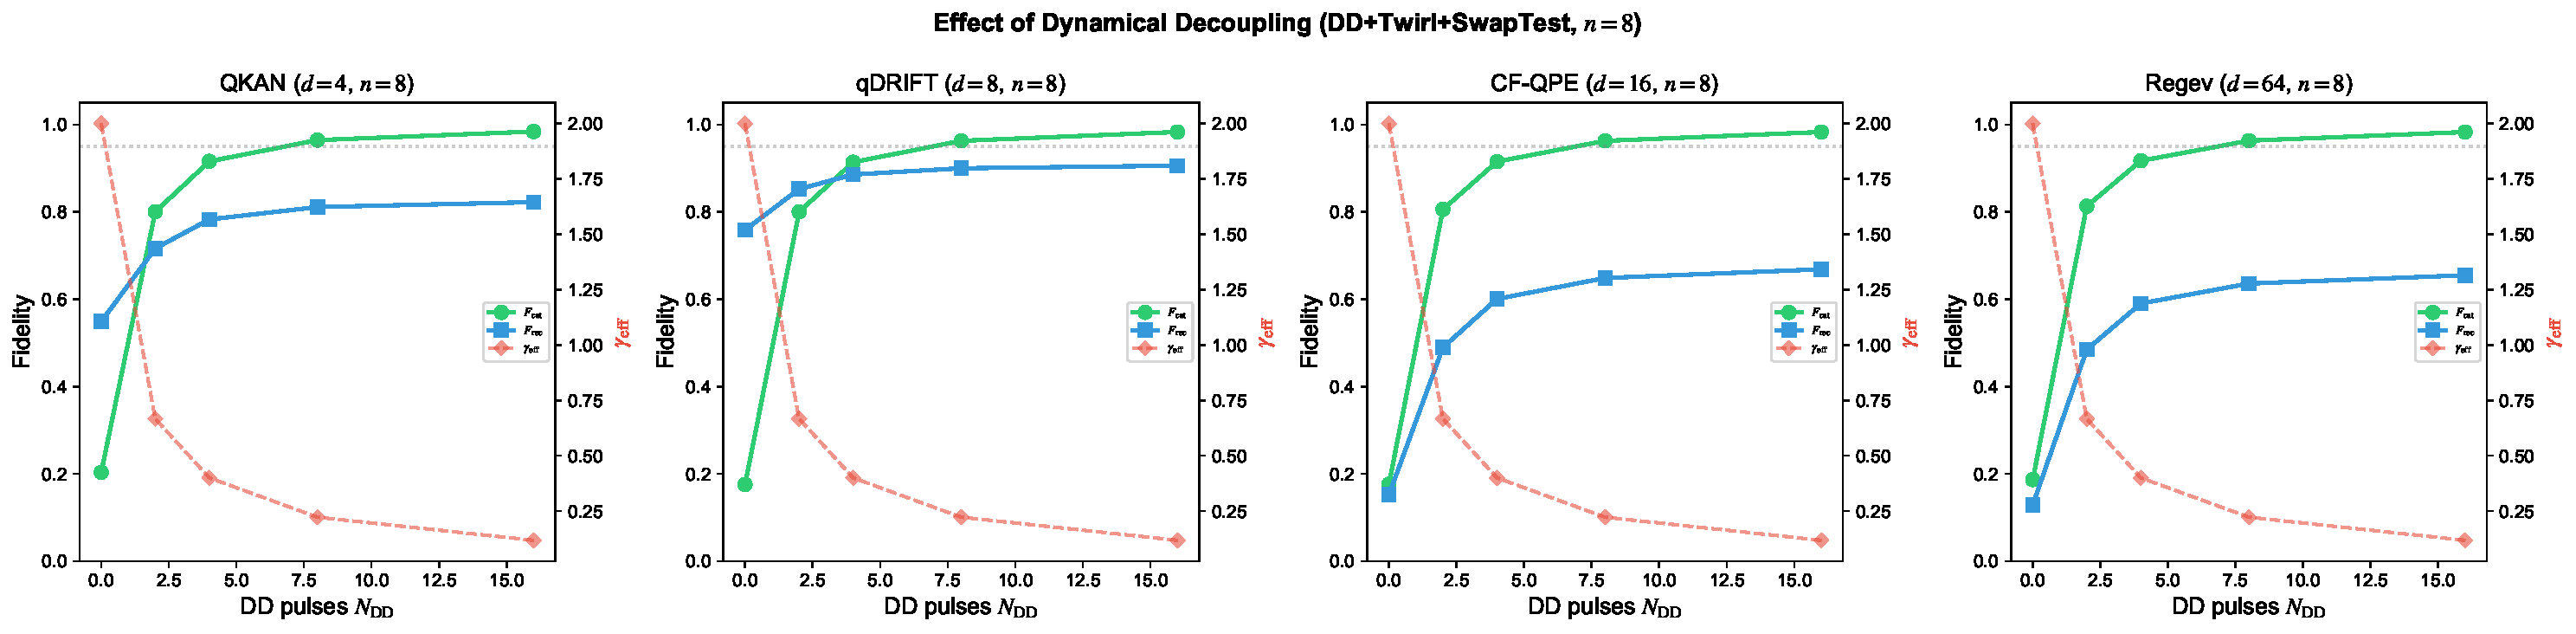
\includegraphics[width=\columnwidth]{fig_dd_sweep}
\caption{Catalyst fidelity vs.\ CPMG pulse count for qDRIFT ($d = 8$, $n = 8$ copies, $\gamma = 2$). DD reduces the effective dephasing, and twirling converts the residual dephasing to depolarizing noise, enabling the swap test to purify efficiently.}
\label{fig:dd_sweep}
\end{figure}

\subsection{Clifford twirling}
\label{sec:twirling}

After DD reduces $\gamma$ to $\gamma_\mathrm{eff}$, the residual noise is still anisotropic dephasing.
Clifford twirling~\cite{Wallman2016} converts any noise channel into a depolarizing channel by averaging over random Clifford gates: for each noisy copy, a random Clifford $C$ is applied before the noise and $C^\dagger$ after, and the average over the Clifford group yields
\begin{equation}
\overline{\mathcal{E}}_\mathrm{twirl}(\rho) = (1 - p_\mathrm{eff})\rho + p_\mathrm{eff}\, \frac{I}{d},
\label{eq:twirl}
\end{equation}
where the effective depolarizing parameter is determined by the average fidelity $\bar{F}$ of the original channel:
\begin{equation}
p_\mathrm{eff} = 1 - \frac{d\, \bar{F}_\mathrm{avg} - 1}{d - 1}.
\label{eq:p_eff}
\end{equation}
For dephasing with strength $\gamma_\mathrm{eff}$ and $H_S = \mathrm{diag}(0, 1, \ldots, d-1)$, the average fidelity is $\bar{F}_\mathrm{avg} = d^{-2}\sum_{i,j} e^{-\gamma_\mathrm{eff}|E_i - E_j|}$.
The twirling converts the exponentially non-uniform dephasing profile into a single depolarizing parameter $p_\mathrm{eff}$, which the swap test handles efficiently.

\subsection{Combined pipeline: DD $\to$ Twirl $\to$ Swap Test}
\label{sec:pipeline}

The full pipeline operates in three stages:
\begin{enumerate}
\item \textbf{DD stage}: Apply CPMG-$N$ to each noisy copy, reducing $\gamma \to \gamma_\mathrm{eff} = \gamma/(N+1)$.
\item \textbf{Twirl stage}: Apply Clifford twirling to each DD-protected copy, converting dephasing($\gamma_\mathrm{eff}$) $\to$ depolarizing($p_\mathrm{eff}$).
\item \textbf{Purification stage}: Apply the standard recursive swap test to the twirled copies, exploiting doubly exponential convergence under depolarizing noise.
\end{enumerate}

The physical interpretation is: DD suppresses the noise magnitude, twirling isotropizes the residual noise geometry, and the swap test purifies the isotropic noise efficiently.
Each stage addresses a distinct obstacle---magnitude, anisotropy, and mixedness---and the composition is more effective than any single technique.

Table~\ref{tab:dd_pipeline} presents the main results of the DD~+~Twirl pipeline across all four algorithms with CPMG-8 and $n = 8$ copies.

\begin{table}[tb]
\caption{DD~+~Twirl~+~Swap Test pipeline results (CPMG-8, $\gamma_\mathrm{eff} = 0.222$, $n = 8$ copies, original $\gamma = 2$). ``Raw $F_\mathrm{cat}$'' is the catalyst fidelity without DD or twirling; ``DD+Twirl $F_\mathrm{cat}$'' and ``DD+Twirl $F_\mathrm{rec}$'' are the catalyst and recovery fidelities with the full pipeline.}
\label{tab:dd_pipeline}
\begin{ruledtabular}
\begin{tabular}{lcccc}
Algorithm & $d$ & Raw $F_\mathrm{cat}$ & \makecell{DD+Twirl \\ $F_\mathrm{cat}$} & \makecell{DD+Twirl \\ $F_\mathrm{rec}$} \\
\colrule
QKAN & 4 & 0.351 & 0.964 & 0.811 \\
qDRIFT & 8 & 0.173 & 0.963 & 0.900 \\
CF-QPE & 16 & 0.085 & 0.963 & 0.649 \\
Regev & 64 & 0.021 & 0.963 & 0.636 \\
\end{tabular}
\end{ruledtabular}
\end{table}

The pipeline achieves $F_\mathrm{cat} > 0.96$ uniformly across all dimensions, in stark contrast to the raw swap test ($F_\mathrm{cat} = 0.02$--$0.44$), DD alone ($F_\mathrm{cat} = 0.16$--$0.99$, dimension-dependent), or twirling alone ($F_\mathrm{cat} = 0.18$--$0.21$, which fails because twirling without DD converts strong dephasing into strong depolarizing noise).
The key insight is that neither DD nor twirling alone suffices: DD reduces dephasing magnitude but preserves its anisotropy, while twirling isotropizes noise but does not reduce its magnitude; only the combination followed by purification achieves uniformly high fidelity (Fig.~\ref{fig:dd_pipeline}).

\begin{figure}[tb]
\centering
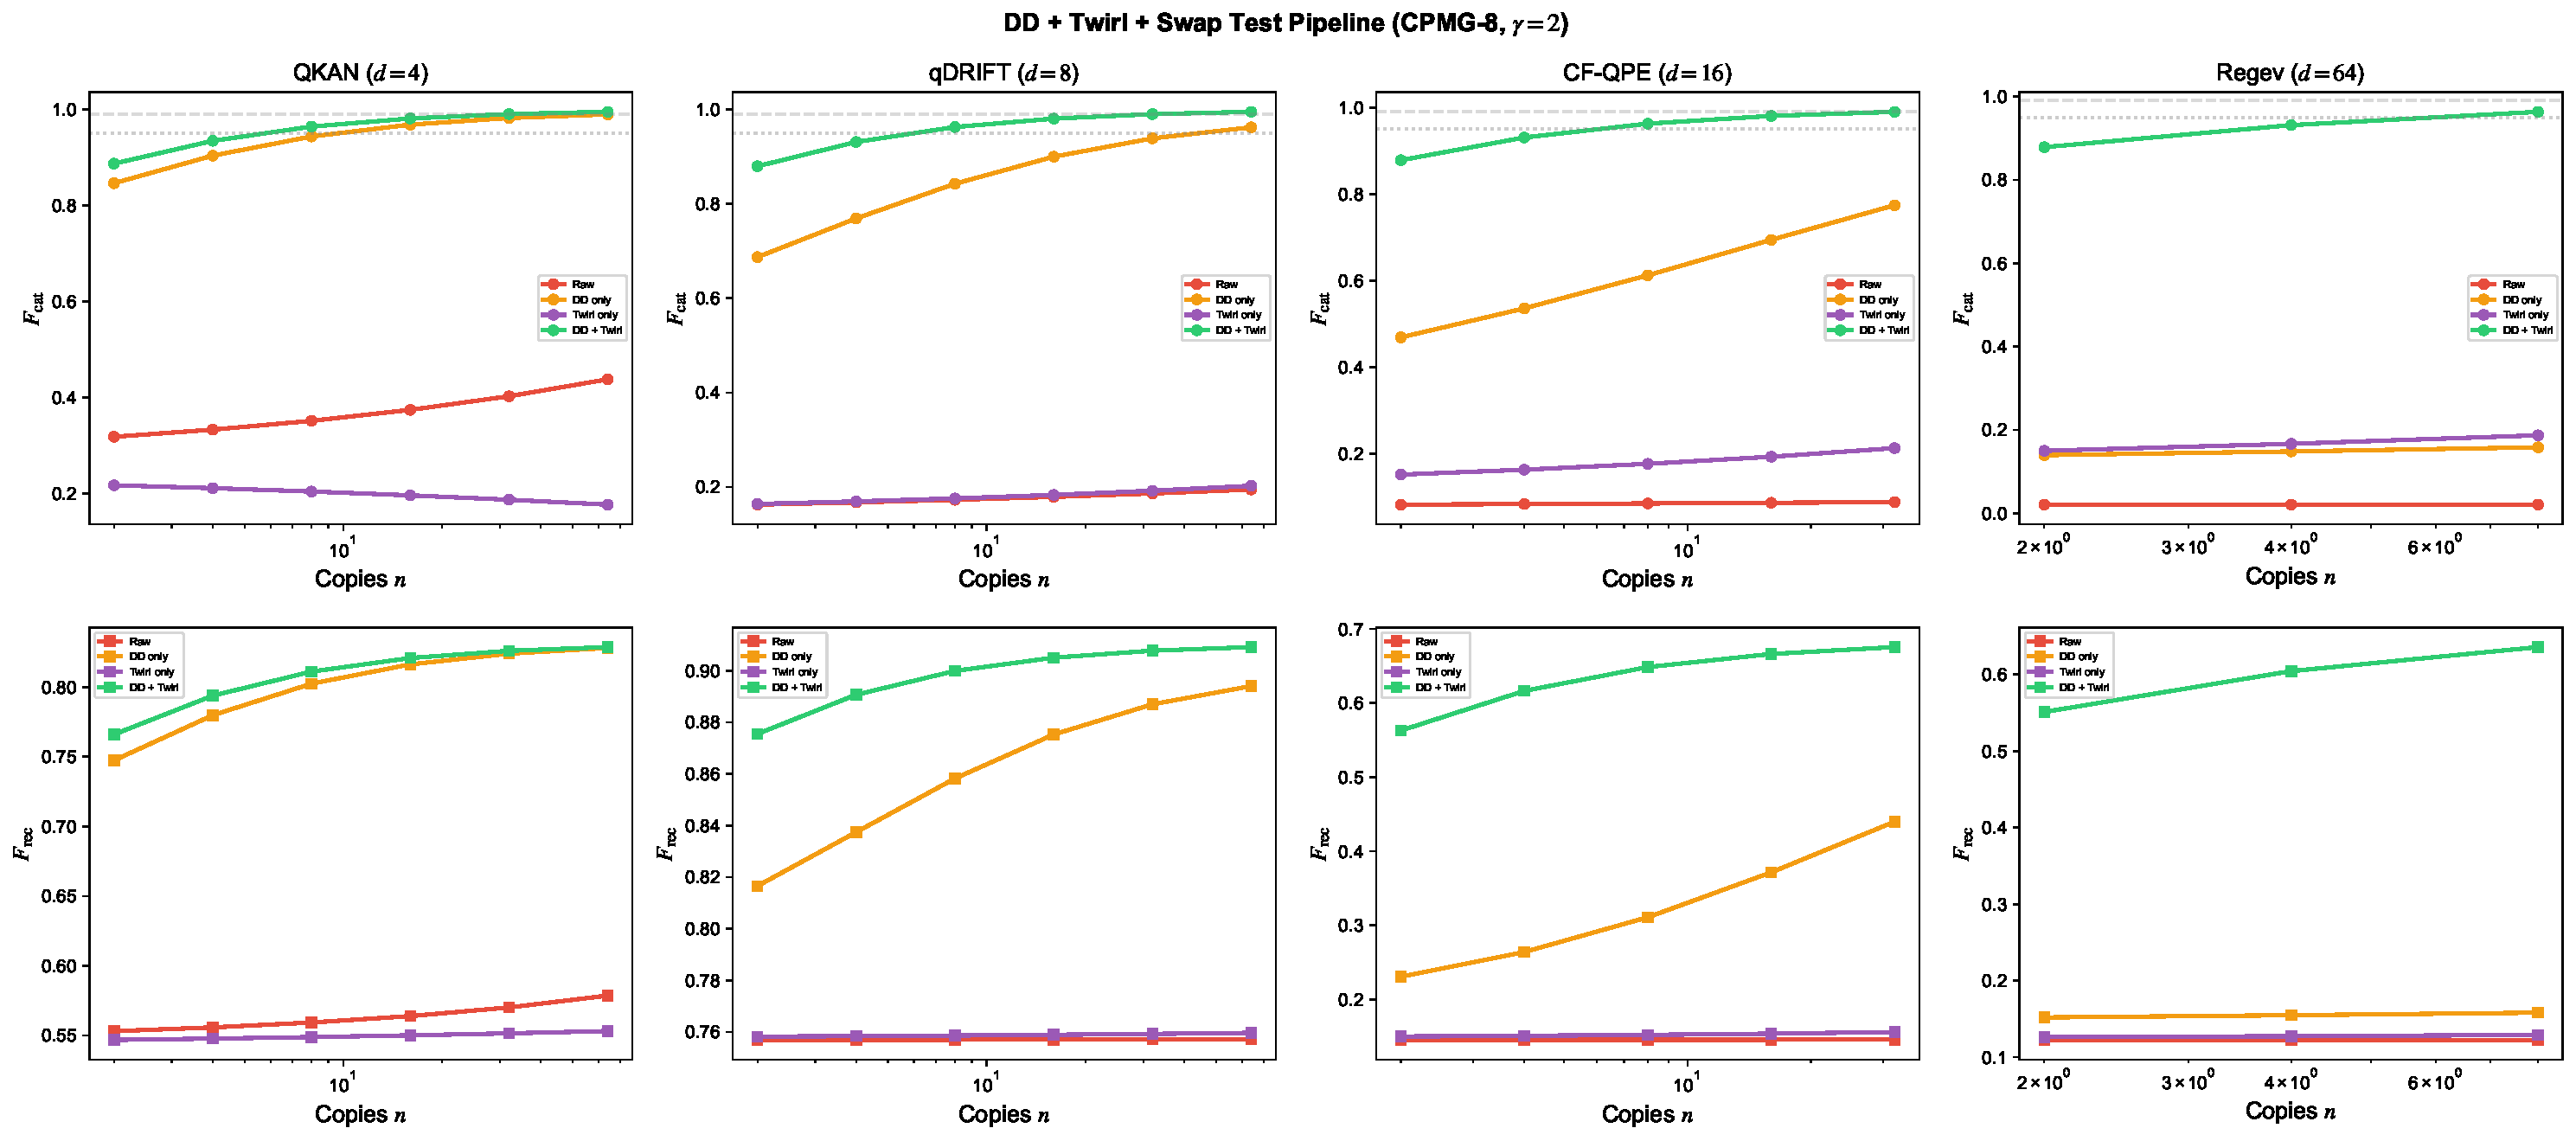
\includegraphics[width=\columnwidth]{fig_dd_pipeline}
\caption{Pipeline comparison under dephasing $\gamma = 2$ with $n = 8$ copies (CPMG-8). Raw purification (red) fails for $d \geq 8$. DD alone (orange) improves but remains dimension-dependent. Twirl alone (purple) fails. DD~+~Twirl (green) achieves $F_\mathrm{cat} > 0.96$ uniformly across all dimensions.}
\label{fig:dd_pipeline}
\end{figure}

\begin{figure}[tb]
\centering
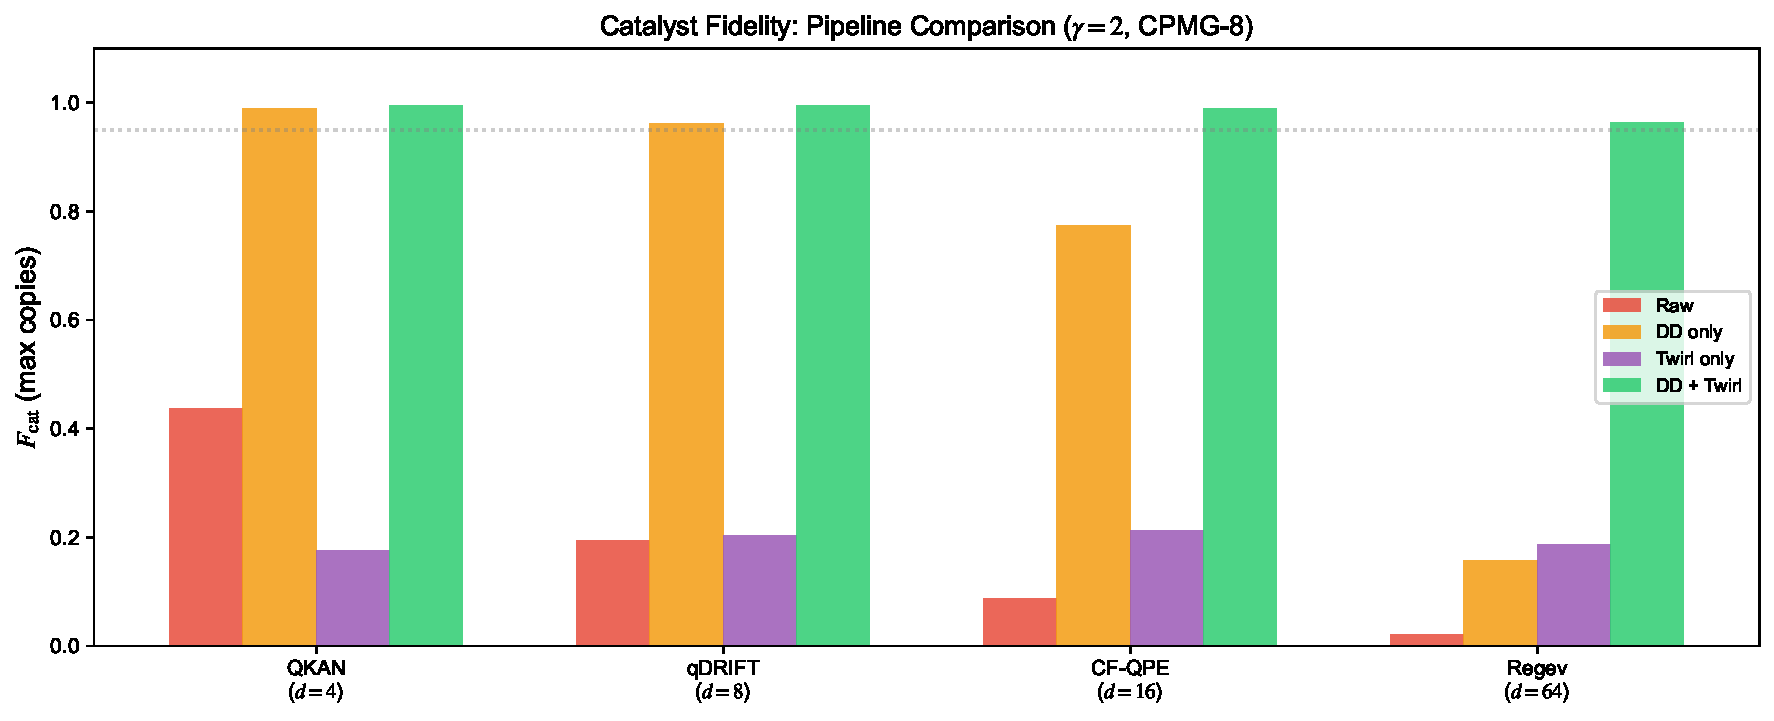
\includegraphics[width=\columnwidth]{fig_dd_summary}
\caption{Summary of all catalyst preparation strategies under dephasing $\gamma = 2$: variational (0 copies), standard swap test, covariant swap test, and DD~+~Twirl~+~Swap Test pipeline (CPMG-8, 8 copies). The DD~+~Twirl pipeline dramatically outperforms all other methods.}
\label{fig:dd_summary}
\end{figure}

The recovery fidelity $F_\mathrm{rec}$ ranges from 0.636 (Regev, $d = 64$) to 0.900 (qDRIFT, $d = 8$), representing a substantial improvement over the raw case where $F_\mathrm{rec} \leq 0.12$ for $d \geq 16$.
The variation in $F_\mathrm{rec}$ across dimensions reflects both the catalyst quality (which is uniform at $F_\mathrm{cat} \approx 0.96$) and the efficiency of the simplified recovery model, which uses fewer EC rotation parameters relative to the Hilbert space dimension at large $d$.

\subsection{Resource cost of the pipeline}
\label{sec:dd_resources}

The total resource cost of the DD~+~Twirl~+~Swap Test pipeline is:
\begin{itemize}
\item $N$ DD pulses per copy (CPMG-8: $N = 8$ $\pi$-pulses per copy).
\item $O(n_q^2)$ Clifford gates per copy for the twirling (single-qubit Cliffords suffice for the $d$-dimensional generalization).
\item $n = 2^k$ copies for $k$ rounds of the swap test (here $k = 3$, $n = 8$).
\end{itemize}
The total copy count is $n = 8$, identical to the raw swap test.
The overhead consists of $8 \times 8 = 64$ additional $\pi$-pulses across all copies, plus $O(n \cdot n_q^2)$ Clifford gates for twirling---negligible compared to the $10^9$-fold reduction in the required copy count relative to distillation.
For a $d = 64$ system ($n_q = 6$), the pipeline requires 8~copies, 64~DD pulses, and $\sim\!288$ Clifford gates, compared to $7.3 \times 10^{10}$ copies for distillation.


%% ============================================================
\section{Unified Benchmark}
\label{sec:benchmark}

\subsection{Algorithm benchmarks}
\label{sec:alg_bench}

We benchmark all three catalyst preparation methods on the four algorithms from Ref.~\cite{Wakaura2026}, using the CQEC recovery pipeline: prepare catalyst $\to$ apply noise to target $\to$ recover.
The recovery fidelity is defined as $F_\mathrm{rec} = \bra{\psi_0}\rho_\mathrm{rec}\ket{\psi_0}$, where $\rho_\mathrm{rec} = \mathrm{Tr}_C[\Lambda(\rho_\mathrm{noisy} \otimes \rho_\mathrm{cat})]$ is the recovered state and $\ket{\psi_0}$ is the original pure target state.
The recovery channel $\Lambda$ uses a simplified model: a single layer of $d-1$ EC rotations $G_{(i,S),(i,C)}(\theta_i, \phi_i)$ coupling system level $\ket{i}_S$ with catalyst level $\ket{i}_C$ for $i = 1, \ldots, d-1$ (i.e., $2(d-1)$ real parameters), with rotation angles chosen to maximize the overlap $\bra{\psi_0}\rho_\mathrm{rec}\ket{\psi_0}$ via gradient-free optimization (Nelder--Mead with 10 random restarts).
This is less powerful than the full variational recovery circuit of Ref.~\cite{Wakaura2026}, and the Nelder--Mead optimizer may converge to local optima rather than the global maximum, so the reported $F_\mathrm{rec}$ values are conservative lower bounds.
Note that the recovery channel $\Lambda$ is a deterministic unitary (no post-selection), so the total post-selection overhead of the full pipeline comes only from the catalyst purification stage.

\begin{table*}[t]
\caption{Catalyst fidelity $F_\mathrm{cat}$ and CQEC recovery fidelity $F_\mathrm{rec}$ under dephasing ($\gamma = 2$). Variational uses zero copies; swap tests use $n$ copies as indicated (parenthetical numbers after $F_\mathrm{cat}$ denote the copy count $n$ used). DD+Twirl uses CPMG-8 with $n = 8$ copies. Distillation $n^*$ is the Shiraishi--Takagi estimate for $F_\mathrm{cat} \geq 0.99$.}
\label{tab:main}
\begin{ruledtabular}
\begin{tabular}{llcccccccccc}
& & \multicolumn{2}{c}{Variational ($n = 0$)} & \multicolumn{2}{c}{Standard ($n_\mathrm{max}$)} & \multicolumn{2}{c}{Covariant ($n_\mathrm{max}$)} & \multicolumn{2}{c}{\textbf{DD+Twirl} ($n = 8$)} & Distillation \\
Algorithm & $d$ & $F_\mathrm{cat}$ & $F_\mathrm{rec}$ & $F_\mathrm{cat}$ & $F_\mathrm{rec}$ & $F_\mathrm{cat}$ & $F_\mathrm{rec}$ & $F_\mathrm{cat}$ & $F_\mathrm{rec}$ & $n^*$ \\
\colrule
QKAN & 4 & 1.000 & 0.83 & 0.438 (64) & 0.579 & 0.411 (64) & 0.573 & \textbf{0.964} & \textbf{0.811} & $7.3 \times 10^5$ \\
qDRIFT & 8 & 0.993 & 0.73 & 0.195 (64) & 0.757 & 0.274 (64) & 0.759 & \textbf{0.963} & \textbf{0.900} & $1.8 \times 10^7$ \\
CF-QPE & 16 & 0.960 & 0.65 & 0.088 (32) & 0.146 & 0.106 (32) & 0.147 & \textbf{0.963} & \textbf{0.649} & $2.9 \times 10^8$ \\
Regev & 64 & --- & --- & 0.021 (8) & 0.123 & 0.022 (8) & 0.123 & \textbf{0.963} & \textbf{0.636} & $7.3 \times 10^{10}$ \\
\end{tabular}
\end{ruledtabular}
\end{table*}

Key observations:
\begin{enumerate}
\item Under strong dephasing ($\gamma = 2$), the standard and covariant swap tests alone fail to achieve high catalyst fidelity. At $d = 64$, the covariant method reaches only $F_\mathrm{cat} = 0.022$ (vs.\ $0.021$ for standard)---barely above the random-guessing baseline $1/d \approx 0.016$.
\item The covariant method provides a modest improvement over the standard swap test: a factor of $1.2$--$1.4\times$ in $F_\mathrm{cat}$ across all tested dimensions.
\item \textbf{The DD~+~Twirl~+~Swap Test pipeline (Sec.~\ref{sec:dd_twirl}) solves the dephasing problem}: with CPMG-8 and $n = 8$ copies, it achieves $F_\mathrm{cat} > 0.96$ uniformly across all dimensions $d = 4$--$64$, with recovery fidelities $F_\mathrm{rec} = 0.64$--$0.90$. This represents a $10^9$-fold improvement over distillation and is the main contribution of this work.
\item Under depolarizing noise (Table~\ref{tab:standard_depol}), both standard and covariant methods achieve $F_\mathrm{cat} > 0.93$ with 8--64 copies, a $10^4$--$10^8$-fold improvement over distillation.
\item At $d = 4$ (QKAN), the variational approach ($F_\mathrm{cat} = 1.000$) remains competitive with DD+Twirl, as the maximally coherent state is exactly preparable by a simple circuit.
\end{enumerate}

We note that the recovery fidelity $F_\mathrm{rec}$ is computed using a simplified recovery model that does not implement full variational EC-gate optimization~\cite{Wakaura2026}.
Under dephasing, both methods yield low $F_\mathrm{rec}$ values ($0.12$--$0.76$), reflecting the poor catalyst quality.
The threshold for useful recovery depends on the application: for quantum algorithm restart (avoiding re-execution), $F_\mathrm{rec} > 0.5$ already provides advantage over random guessing for $d > 2$, while fault-tolerant applications would require $F_\mathrm{rec} > 1 - O(1/d)$.
Only the $d = 4$ and $d = 8$ cases approach the useful-recovery threshold under dephasing; for $d \geq 16$, the catalyst quality is insufficient for practical CQEC recovery.

For completeness, the $\ell_1$-coherence of the covariant-purified catalysts under dephasing ($\gamma = 2$) at maximum tested copy counts remains far below the ideal values $C_{\ell_1}(\ket{+_d}) = d-1$, consistent with the low $F_\mathrm{cat}$ values reported.
The covariant method recovers only a small fraction of the ideal coherence under strong dephasing, confirming that purification-based approaches are insufficient in this regime.

As a naive baseline, one might use an energy eigenstate $\ket{i}$ (zero coherence, $C_{\ell_1} = 0$) as a catalyst, which would give $F_\mathrm{rec} = 1/d$ (random guessing).
Alternatively, a mixture of eigenstates with correct populations but no coherence yields $F_\mathrm{rec}$ slightly above $1/d$ but still far below the CQEC recovery values, confirming that the off-diagonal coherence---not just the population structure---is essential for recovery.

\subsection{Noise model comparison}
\label{sec:noise_comparison}

\begin{table}[tb]
\caption{Covariant catalyst fidelity $F_\mathrm{cat}$ at maximum tested copy count, by noise model.}
\label{tab:noise}
\begin{ruledtabular}
\begin{tabular}{lcccc}
Algorithm & $d$ & Depol. & Deph. & Combined \\
\colrule
QKAN & 4 & 0.818 & 0.411 & 0.610 \\
qDRIFT & 8 & 0.877 & 0.274 & 0.628 \\
CF-QPE & 16 & 0.924 & 0.106 & 0.251 \\
Regev & 64 & 0.963 & 0.022 & 0.039 \\
\end{tabular}
\end{ruledtabular}
\end{table}

Under depolarizing noise, both standard and covariant methods converge rapidly, with the covariant method reaching $F_\mathrm{cat} > 0.85$ at all tested dimensions using 2--64~copies.
Under dephasing, both methods perform poorly, with $F_\mathrm{cat}$ decreasing sharply with dimension ($F_\mathrm{cat} = 0.022$ at $d = 64$).
The contrast between depolarizing and dephasing performance is stark: at $d = 64$, $F_\mathrm{cat}$ drops from $0.963$ (depolarizing) to $0.022$ (dephasing) for the covariant method alone, highlighting that dephasing is the fundamentally harder noise channel for direct purification-based catalyst preparation.
The DD~+~Twirl pipeline (Sec.~\ref{sec:dd_twirl}) addresses this gap, achieving $F_\mathrm{cat} > 0.96$ under dephasing by converting it to effective depolarizing noise.
Combined noise (dephasing $\gamma = 1$ + depolarizing $p = 0.15$ + amplitude damping $\gamma_\mathrm{AD} = 0.1$) produces intermediate results dominated by the dephasing component, particularly at large $d$.

We note that Yao~\emph{et~al.}~\cite{Yao2025} established optimal probabilistic purification bounds via semidefinite programming for the standard (non-covariant) setting.
Their optimal fidelity for $n$ copies of a depolarized state provides an upper bound for the standard swap test, which our standard swap-test results approach but do not saturate (as the recursive binary-tree protocol is not SDP-optimal).
The covariant swap test operates in a different regime---constrained to energy-conserving operations---so the Yao~\emph{et~al.}\ bounds do not directly apply.
Establishing optimal purification bounds under covariance constraints is an interesting open problem.

We also note the distinction from virtual distillation~\cite{Huggins2021}, which uses $M$ copies of a noisy state to estimate expectation values with exponentially suppressed bias ($\propto \lambda_2^M/\lambda_1^M$) but does not produce a physical purified state.
CQEC requires a physical catalyst state with high coherence, not just error-mitigated expectation values, so virtual distillation is not directly applicable to catalyst preparation.
However, a hybrid approach using virtual distillation to verify catalyst quality without consuming the catalyst could be valuable in practice.

\subsection{Resource--fidelity landscape}
\label{sec:landscape}

Figure~\ref{fig:landscape} presents the unified resource--fidelity comparison.

\begin{figure}[tb]
\centering
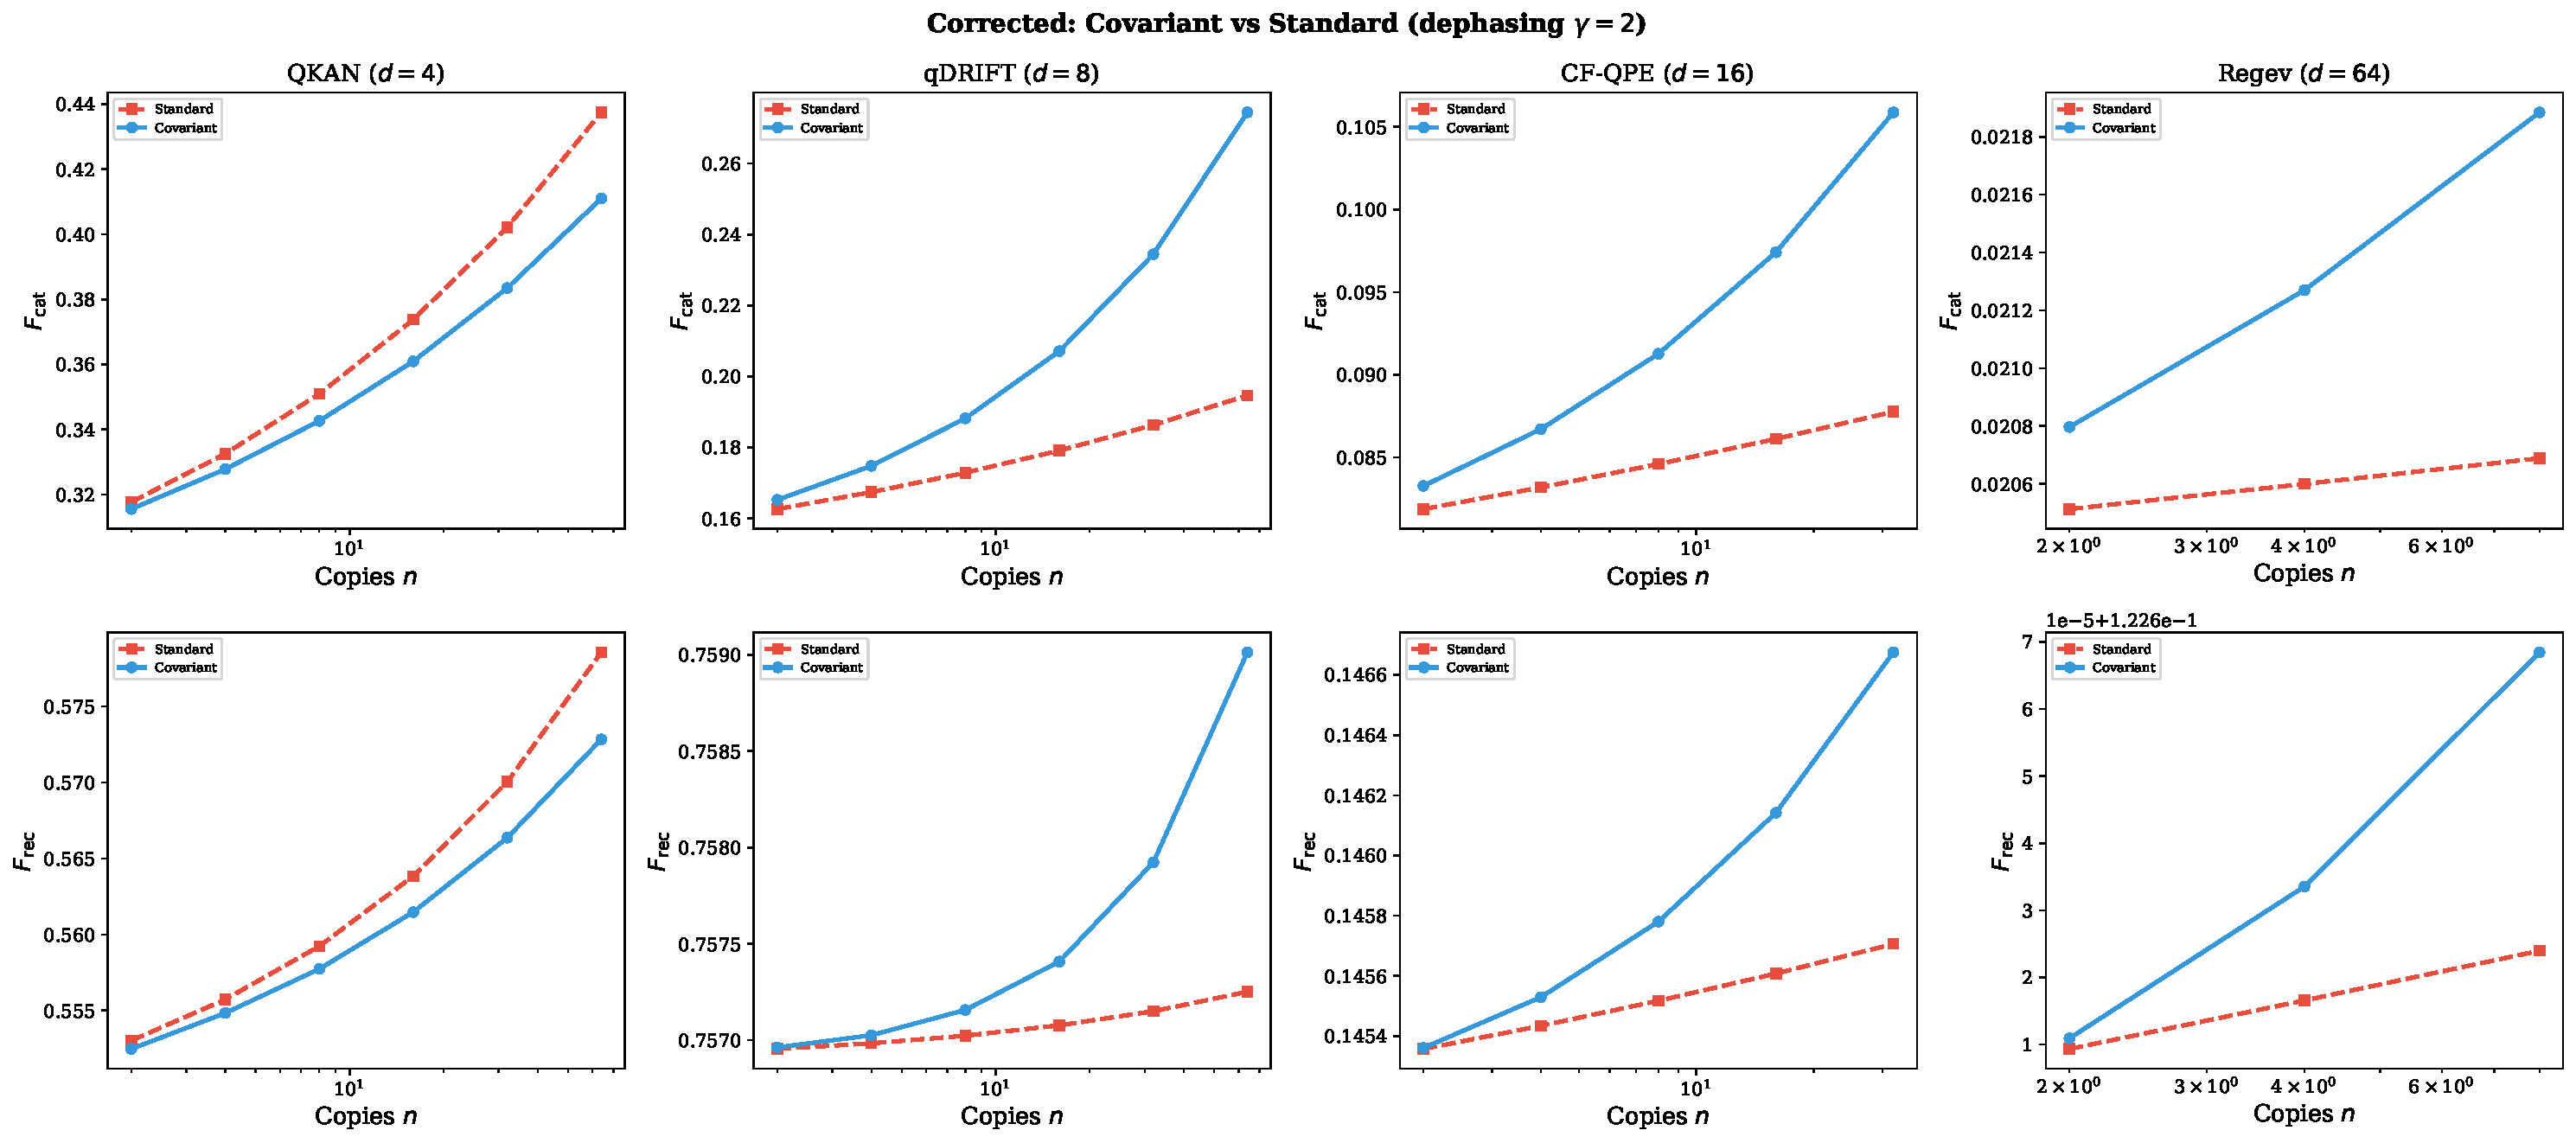
\includegraphics[width=\columnwidth]{fig_covariant_algorithms}
\caption{Catalyst fidelity (top) and CQEC recovery fidelity (bottom) vs.\ copy count under dephasing ($\gamma = 2$) for all four algorithms. Blue: covariant recursive. Red: standard recursive. Both methods perform poorly under strong dephasing, with the covariant method achieving a modest improvement.}
\label{fig:landscape}
\end{figure}

\subsection{Scaling analysis}
\label{sec:scaling}

The copy-count scaling for the four approaches is as follows:
\begin{itemize}
\item \textbf{Distillation}: The theoretical bound gives $n^* \sim C^2/\delta^2$ with $C \sim d^2 e^{\gamma}$ (Ref.~\cite{Shiraishi2024}), yielding $n^* \sim d^4 e^{2\gamma}/\delta^2$.  A numerical fit to the data in Table~\ref{tab:bottleneck} gives $n^* \approx 0.53\, d^{4.12}\, e^{2\gamma}/\delta^2$, consistent with the $d^4$ theoretical scaling.
\item \textbf{Standard swap}: $n \sim 2^{k}$ copies.  Under depolarizing noise, the doubly exponential convergence $\delta_k \sim \delta^{2^k}$ means $k = 3$ rounds ($n = 8$ copies) typically suffice for $F_\mathrm{cat} > 0.93$ across all tested $d$.  Under dephasing ($\gamma = 2$), $F_\mathrm{cat} < 0.44$ for all tested $k$ and $d$.
\item \textbf{Covariant swap}: $n \sim 2^k$ with $k \sim 2$--$3$ rounds for all tested $d$ up to 64. Modest $1.2$--$1.4\times$ improvement over standard under dephasing.
\item \textbf{DD~+~Twirl~+~Swap Test}: $n \sim 2^k$ copies plus $N$ DD pulses and Clifford twirling per copy. With CPMG-8 ($N = 8$) and $k = 3$ ($n = 8$), achieves $F_\mathrm{cat} > 0.96$ under dephasing $\gamma = 2$ for all tested $d$ up to 64. The overhead of $N$ DD pulses per copy is independent of $d$, so the scaling with dimension is the same as the standard swap test under depolarizing noise.
\end{itemize}

Under dephasing ($\gamma = 2$), neither the standard nor the covariant swap test alone achieves $F_\mathrm{cat} \geq 0.5$ at any tested dimension $d \geq 4$, regardless of copy count.
However, the DD~+~Twirl pipeline lifts the effective noise into the depolarizing regime, where the swap test converges rapidly.
Under depolarizing noise, both standard and covariant methods easily achieve $F_\mathrm{cat} > 0.93$ with 8--64 copies, representing a dramatic improvement over distillation.


\subsection{Fidelity vs.\ error strength}
\label{sec:fid_vs_error}

Figure~\ref{fig:fid_vs_error} shows how catalyst fidelity degrades with increasing noise strength at a fixed copy budget of $n = 8$.

\begin{figure}[tb]
\centering
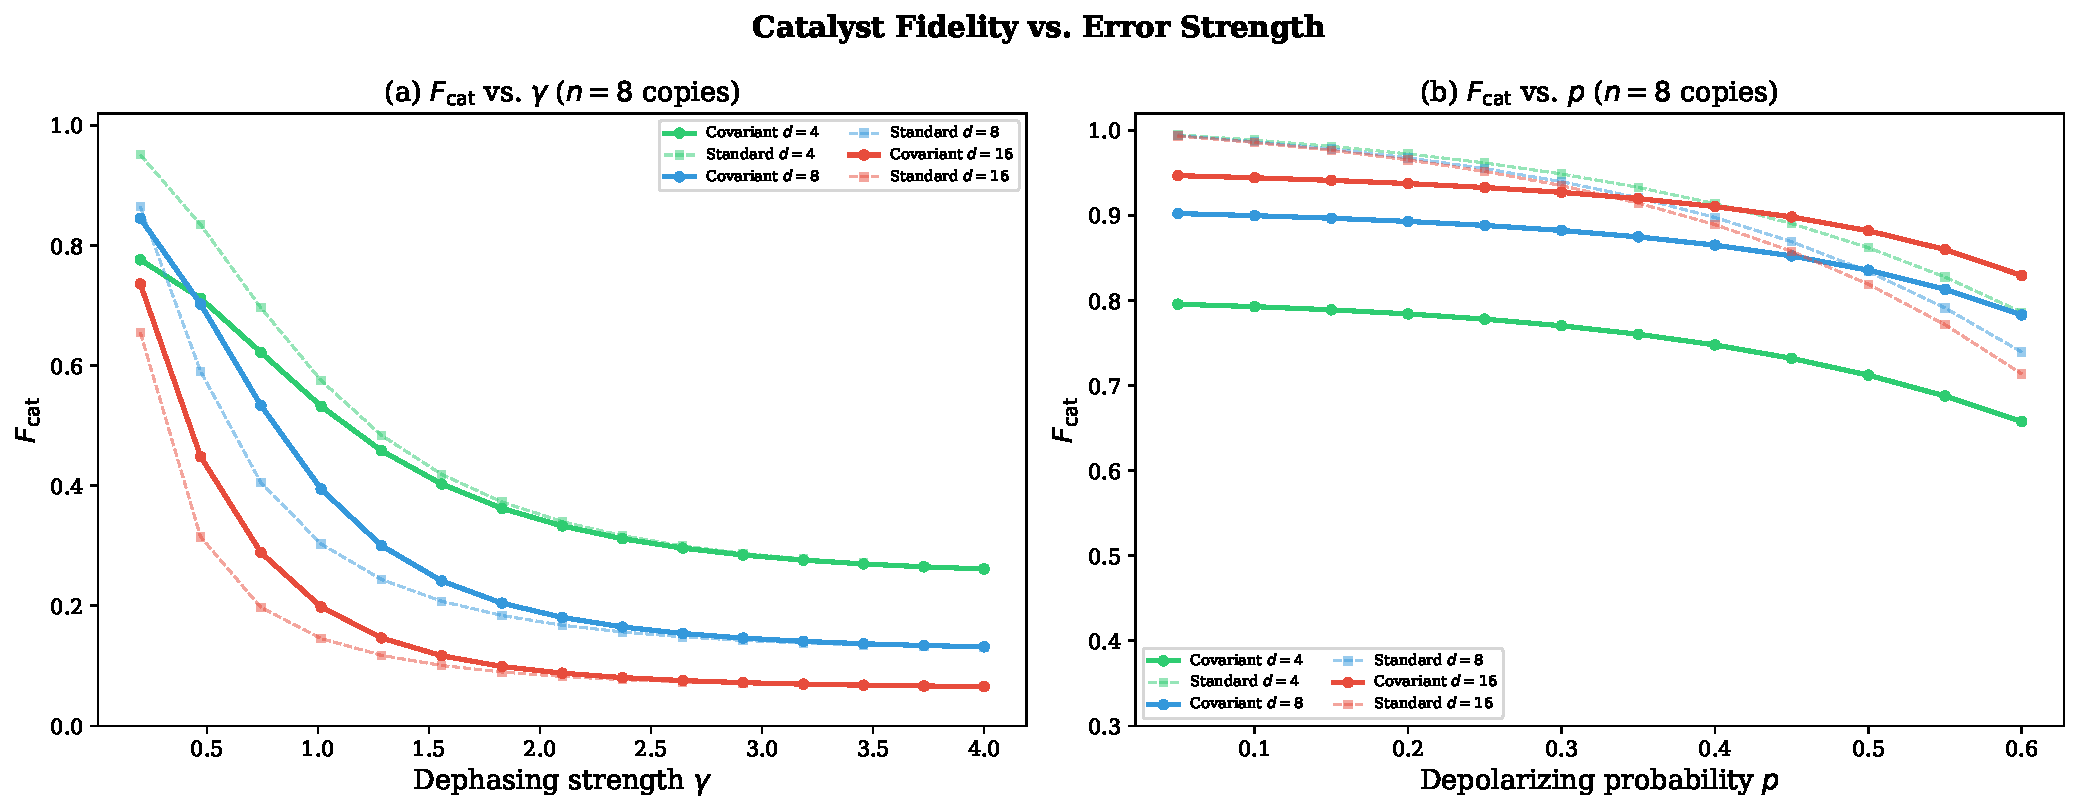
\includegraphics[width=\columnwidth]{fig_fidelity_vs_error}
\caption{Catalyst fidelity vs.\ error strength at $n = 8$ copies.
(a)~Dephasing: $F_\mathrm{cat}$ decreases rapidly with $\gamma$ for all $d$; covariant is slightly better than standard for $d \geq 8$ but the difference is modest.
(b)~Depolarizing: standard achieves $F_\mathrm{cat} > 0.8$ up to $p \approx 0.5$ for all $d$; covariant matches or exceeds standard at $d \geq 8$.}
\label{fig:fid_vs_error}
\end{figure}

Under dephasing [Fig.~\ref{fig:fid_vs_error}(a)], the dominant trend is the rapid decay of $F_\mathrm{cat}$ with $\gamma$ for all dimensions and both methods.
For $d = 8$ and $d = 16$, the covariant method maintains a slightly higher fidelity than the standard method across the full $\gamma$ range, with the gap largest at moderate noise ($\gamma \sim 1$).
At $d = 4$, the two methods are essentially equivalent.
At $\gamma = 2$ (the operating point used throughout this paper), $F_\mathrm{cat} < 0.2$ for $d = 8$ and $F_\mathrm{cat} < 0.1$ for $d = 16$ regardless of method, confirming that strong dephasing is the primary obstacle to purification-based catalyst preparation.
For weaker dephasing ($\gamma \lesssim 0.5$), both methods achieve $F_\mathrm{cat} > 0.7$ for $d \leq 16$, indicating that the purification approach is effective for moderately noisy systems.

Under depolarizing noise [Fig.~\ref{fig:fid_vs_error}(b)], the standard swap test achieves uniformly high fidelity ($F_\mathrm{cat} > 0.8$) up to $p \approx 0.4$, with performance nearly independent of $d$.
The covariant method shows comparable performance at $d = 8$ and $d = 16$ but is slightly inferior at $d = 4$.


\subsection{Fidelity vs.\ system size}
\label{sec:fid_vs_qubits}

Figure~\ref{fig:fid_vs_qubits} shows how catalyst fidelity scales with the number of qubits.

\begin{figure}[tb]
\centering
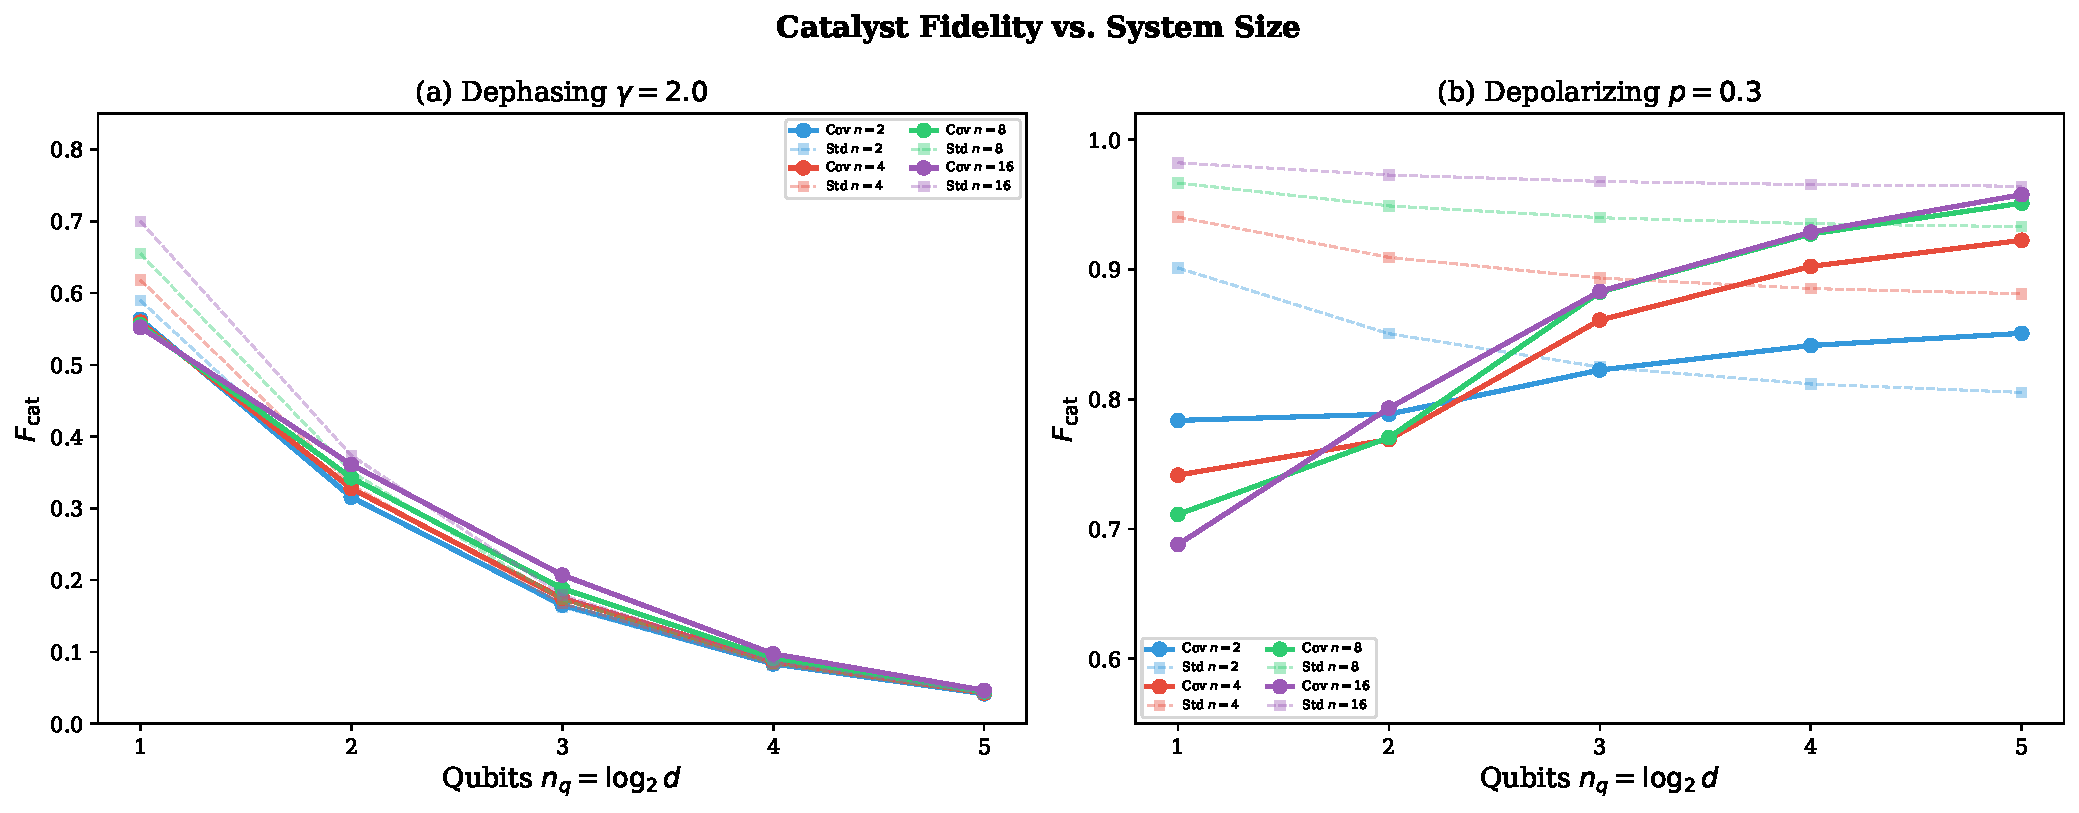
\includegraphics[width=\columnwidth]{fig_fidelity_vs_qubits}
\caption{Catalyst fidelity vs.\ number of qubits $n_q = \log_2 d$ at fixed noise.
(a)~Dephasing $\gamma = 2$: both methods degrade rapidly with system size; $F_\mathrm{cat} < 0.1$ for $n_q \geq 4$.
(b)~Depolarizing $p = 0.3$: standard is nearly dimension-independent; covariant improves with $d$ for $n_q \geq 3$.}
\label{fig:fid_vs_qubits}
\end{figure}

Under dephasing [Fig.~\ref{fig:fid_vs_qubits}(a)], both methods degrade monotonically with system size: $F_\mathrm{cat}$ drops from $\sim 0.5$--$0.7$ at $n_q = 1$ to $\sim 0.04$--$0.05$ at $n_q = 5$.
The covariant method maintains a small advantage over the standard method at each dimension, but the absolute fidelity is far too low for practical catalyst use at $n_q \geq 3$.

Under depolarizing noise [Fig.~\ref{fig:fid_vs_qubits}(b)], the scaling behavior is qualitatively different.
The standard swap test is nearly dimension-independent ($F_\mathrm{cat} \approx 0.93$--$0.97$ at $n = 16$ for all $d$), reflecting the fact that depolarizing noise is a symmetric channel whose error parameter is independent of energy structure.
The covariant method improves with dimension for $n_q \geq 3$, reaching $F_\mathrm{cat} = 0.98$ at $n_q = 5$ vs.\ $F_\mathrm{cat} = 0.64$ at $n_q = 1$ (at $n = 16$).
This improvement arises because larger energy sectors provide more states for intra-sector purification.
However, at $n_q \leq 2$, the covariant method underperforms standard due to sector fragmentation (Sec.~\ref{sec:d4}).


\subsection{Fidelity vs.\ copy count}
\label{sec:fid_vs_copies}

Figure~\ref{fig:fid_vs_copies} presents the convergence of catalyst fidelity with increasing copy count.

\begin{figure}[tb]
\centering
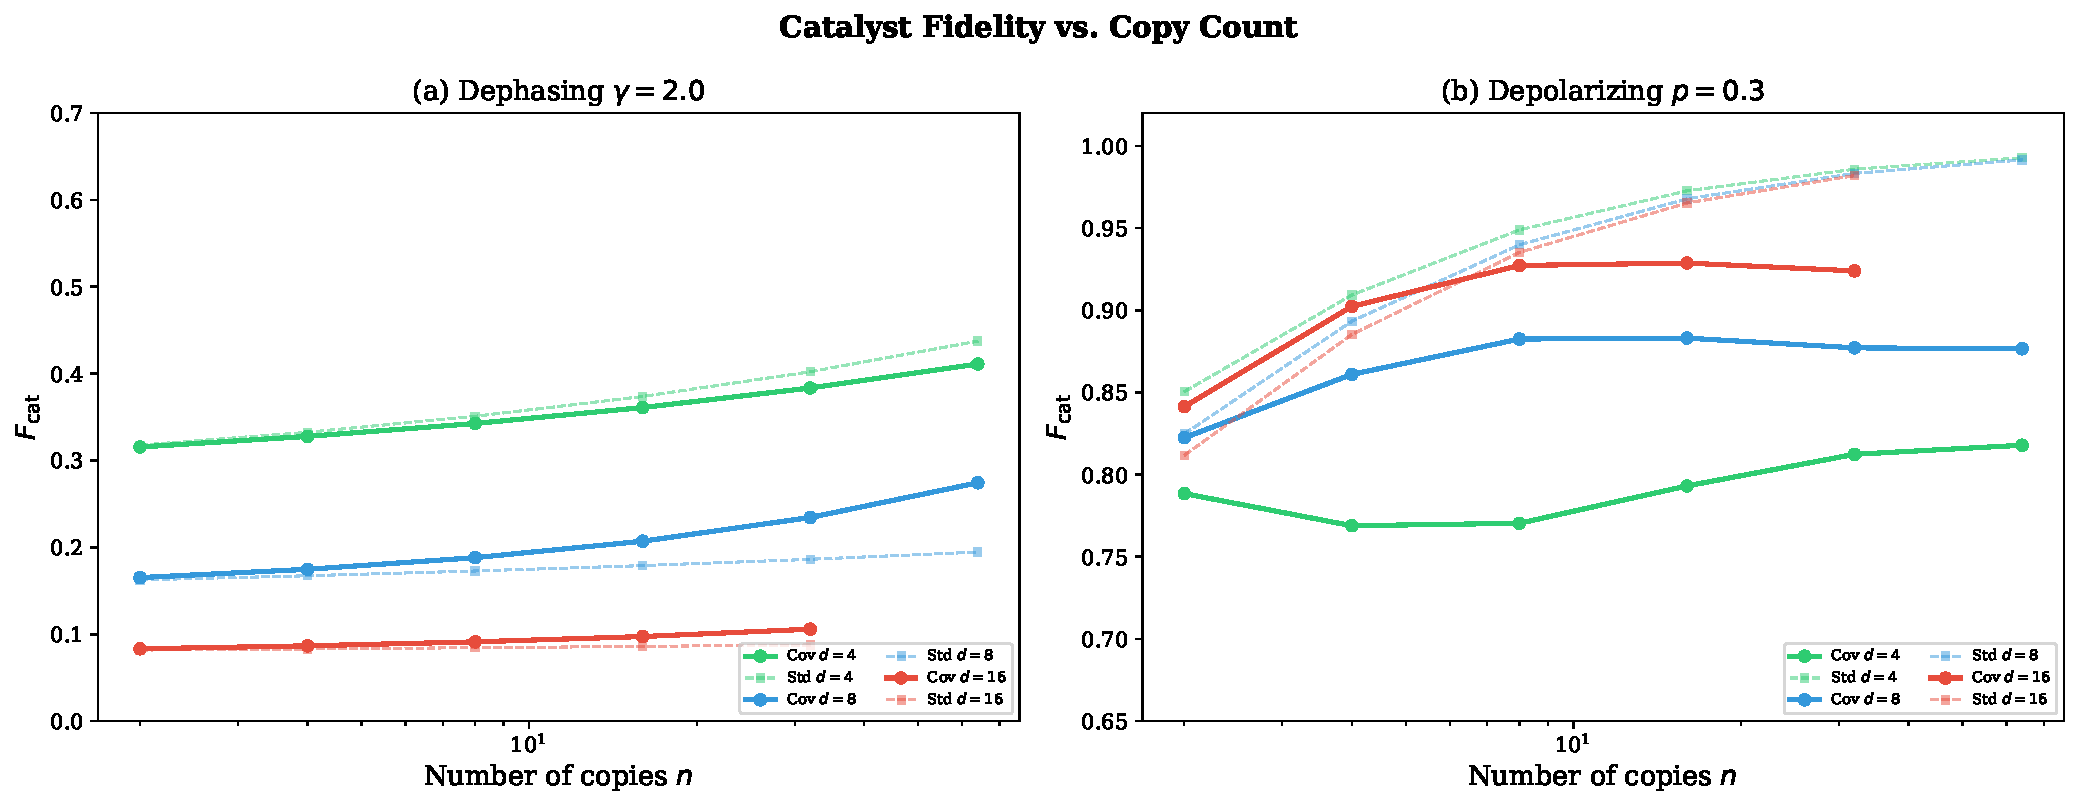
\includegraphics[width=\columnwidth]{fig_fidelity_vs_copies}
\caption{Catalyst fidelity vs.\ copy count $n$ for $d = 4, 8, 16$.
(a)~Dephasing $\gamma = 2$: slow logarithmic improvement; covariant is better for $d = 8$ but the gap is modest.
(b)~Depolarizing $p = 0.3$: rapid doubly exponential convergence to $F_\mathrm{cat} \to 1$; standard achieves $F_\mathrm{cat} > 0.99$ by $n = 64$.}
\label{fig:fid_vs_copies}
\end{figure}

Under dephasing [Fig.~\ref{fig:fid_vs_copies}(a)], both methods show slow, logarithmic improvement with copy count.
For $d = 8$, the covariant method reaches $F_\mathrm{cat} = 0.27$ at $n = 64$ (vs.\ $0.19$ for standard), while for $d = 4$ the two methods are comparable ($F_\mathrm{cat} \approx 0.41$--$0.44$).
The slow convergence under dephasing contrasts sharply with the depolarizing case and reflects the fundamental difficulty: dephasing destroys the relative phase information that the swap test's symmetric projection is designed to recover, and neither the global nor sector-wise symmetric projection can efficiently restore strongly dephased coherence from a small number of copies.

Under depolarizing noise [Fig.~\ref{fig:fid_vs_copies}(b)], the standard swap test shows rapid doubly exponential convergence, reaching $F_\mathrm{cat} > 0.99$ by $n = 64$ for all tested $d$.
The covariant method converges more slowly under depolarizing noise, reaching $F_\mathrm{cat} \approx 0.82$--$0.92$ at $n = 64$.
This confirms that the standard swap test, which exploits the full symmetric subspace, is better suited for symmetric (depolarizing) noise, while the covariant sector-wise approach is optimized for anisotropic (dephasing) noise.


\subsection{Fidelity vs.\ error strength}
\label{sec:fid_vs_error}

Figure~\ref{fig:fid_vs_error} presents the catalyst fidelity as a function of noise strength for both dephasing and depolarizing channels, at fixed copy count $n = 8$ (3~rounds).

\begin{figure}[tb]
\centering
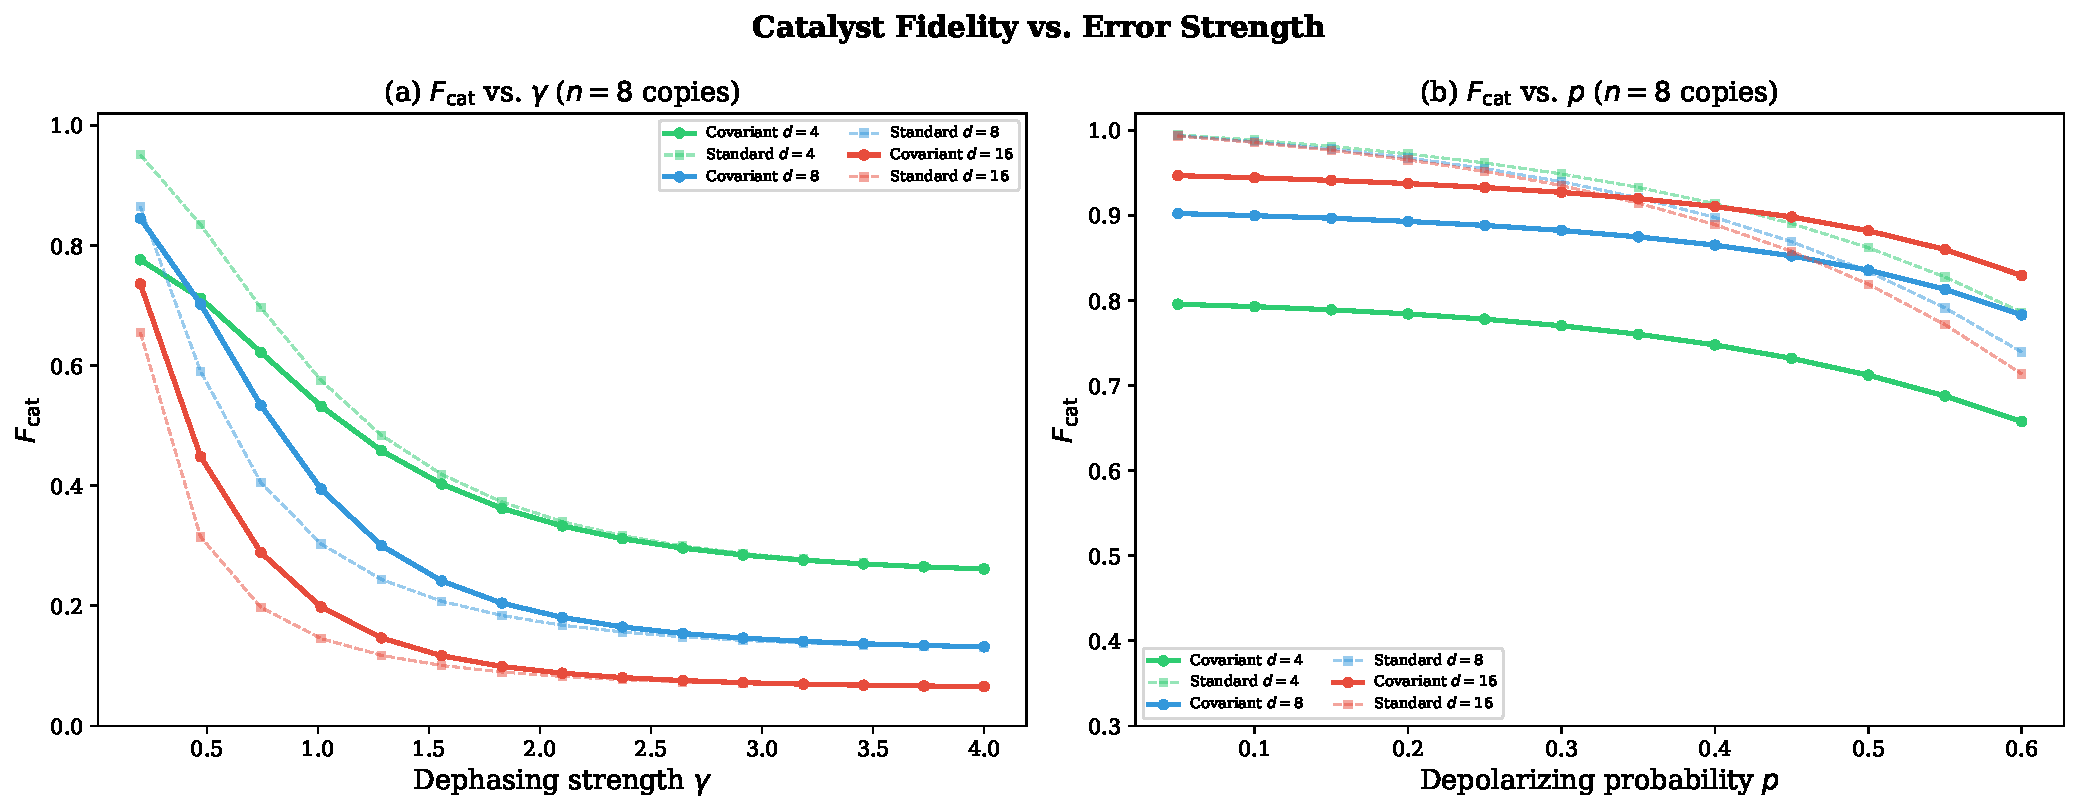
\includegraphics[width=\columnwidth]{fig_fidelity_vs_error}
\caption{Catalyst fidelity vs.\ error strength at $n = 8$ copies.
(a)~Dephasing $\gamma \in [0.2, 4.0]$: both covariant (solid) and standard (dashed) methods degrade rapidly with increasing $\gamma$, with the covariant method modestly better.
(b)~Depolarizing $p \in [0.05, 0.6]$: both methods perform comparably, with standard slightly better at $d = 4$.}
\label{fig:fid_vs_error}
\end{figure}

Under dephasing [Fig.~\ref{fig:fid_vs_error}(a)], both methods degrade rapidly with increasing $\gamma$.
The covariant method is modestly better than the standard method across the tested range, but neither achieves $F_\mathrm{cat} > 0.5$ at $\gamma = 2$ for $d \geq 8$.
At very strong dephasing ($\gamma > 3$), both methods converge to $F_\mathrm{cat} \to 1/d$ as coherence is exponentially suppressed.

Under depolarizing noise [Fig.~\ref{fig:fid_vs_error}(b)], the two methods achieve comparable fidelity across all tested dimensions.
The standard method is marginally better at $d = 4$ because the global symmetric projection has higher dimension than the sector-wise projections (Sec.~\ref{sec:d4}).
For $d \geq 8$, the covariant method matches or slightly exceeds standard performance, confirming that the sector-wise approach incurs no penalty when dephasing is absent.


\subsection{Fidelity vs.\ system size}
\label{sec:fid_vs_qubits}

Figure~\ref{fig:fid_vs_qubits} shows the catalyst fidelity as a function of system size under both noise models.

\begin{figure}[tb]
\centering
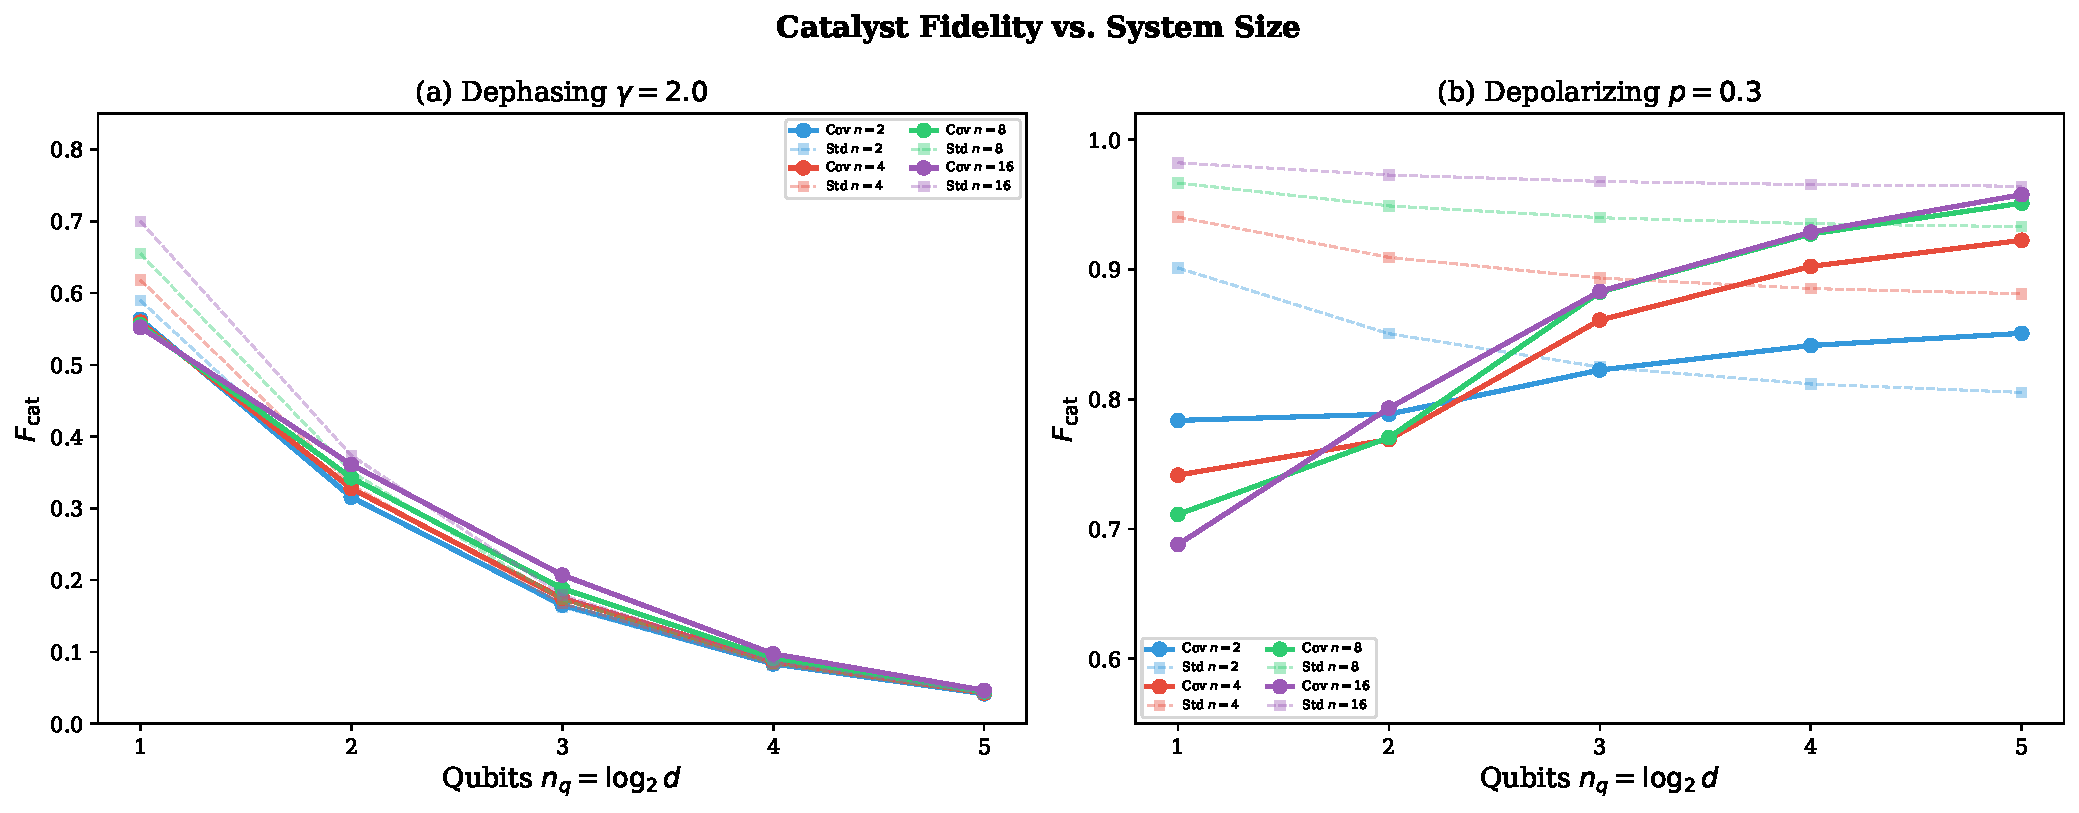
\includegraphics[width=\columnwidth]{fig_fidelity_vs_qubits}
\caption{Catalyst fidelity vs.\ number of qubits $n_q = \log_2 d$ at fixed noise.
(a)~Dephasing $\gamma = 2.0$: both covariant (solid, circles) and standard (dashed, squares) methods degrade rapidly with system size, with $F_\mathrm{cat} \to 1/d$ at large $d$.
The covariant method is modestly better ($1.2$--$1.4\times$).
(b)~Depolarizing $p = 0.3$: both methods perform well, with mild degradation at larger qubit count.}
\label{fig:fid_vs_qubits}
\end{figure}

Under dephasing [Fig.~\ref{fig:fid_vs_qubits}(a)], both methods degrade rapidly with system size.
At $d = 64$ ($n_q = 6$), both methods produce catalysts with fidelity near $1/d$, indicating that strong dephasing overwhelms the purification protocol.
The covariant method consistently achieves slightly higher fidelity than the standard swap test, but the improvement is modest and insufficient for practical CQEC recovery at large $d$.

Under depolarizing noise [Fig.~\ref{fig:fid_vs_qubits}(b)], both methods show mild degradation with system size, as expected from the depolarizing error parameter $\delta$ being independent of the energy structure.
The covariant and standard methods achieve comparable fidelity, confirming that the covariant advantage is specific to coherence-anisotropic noise channels such as dephasing, though even in that case the advantage is quantitatively small.

These results for the standard and covariant methods alone identify dephasing-dominated noise at large $d$ as the most challenging regime.
The DD~+~Twirl pipeline (Sec.~\ref{sec:dd_twirl}) addresses this by converting dephasing to depolarizing noise before purification, as quantified in the following three subsections.


\subsection{DD+Twirl: fidelity vs.\ error strength}
\label{sec:dd_fid_vs_error}

Figure~\ref{fig:dd_vs_error} compares raw dephasing and the DD+Twirl pipeline across dephasing strengths $\gamma \in [0.1, 4.0]$ at fixed $n = 8$ copies.

\begin{figure}[tb]
\centering
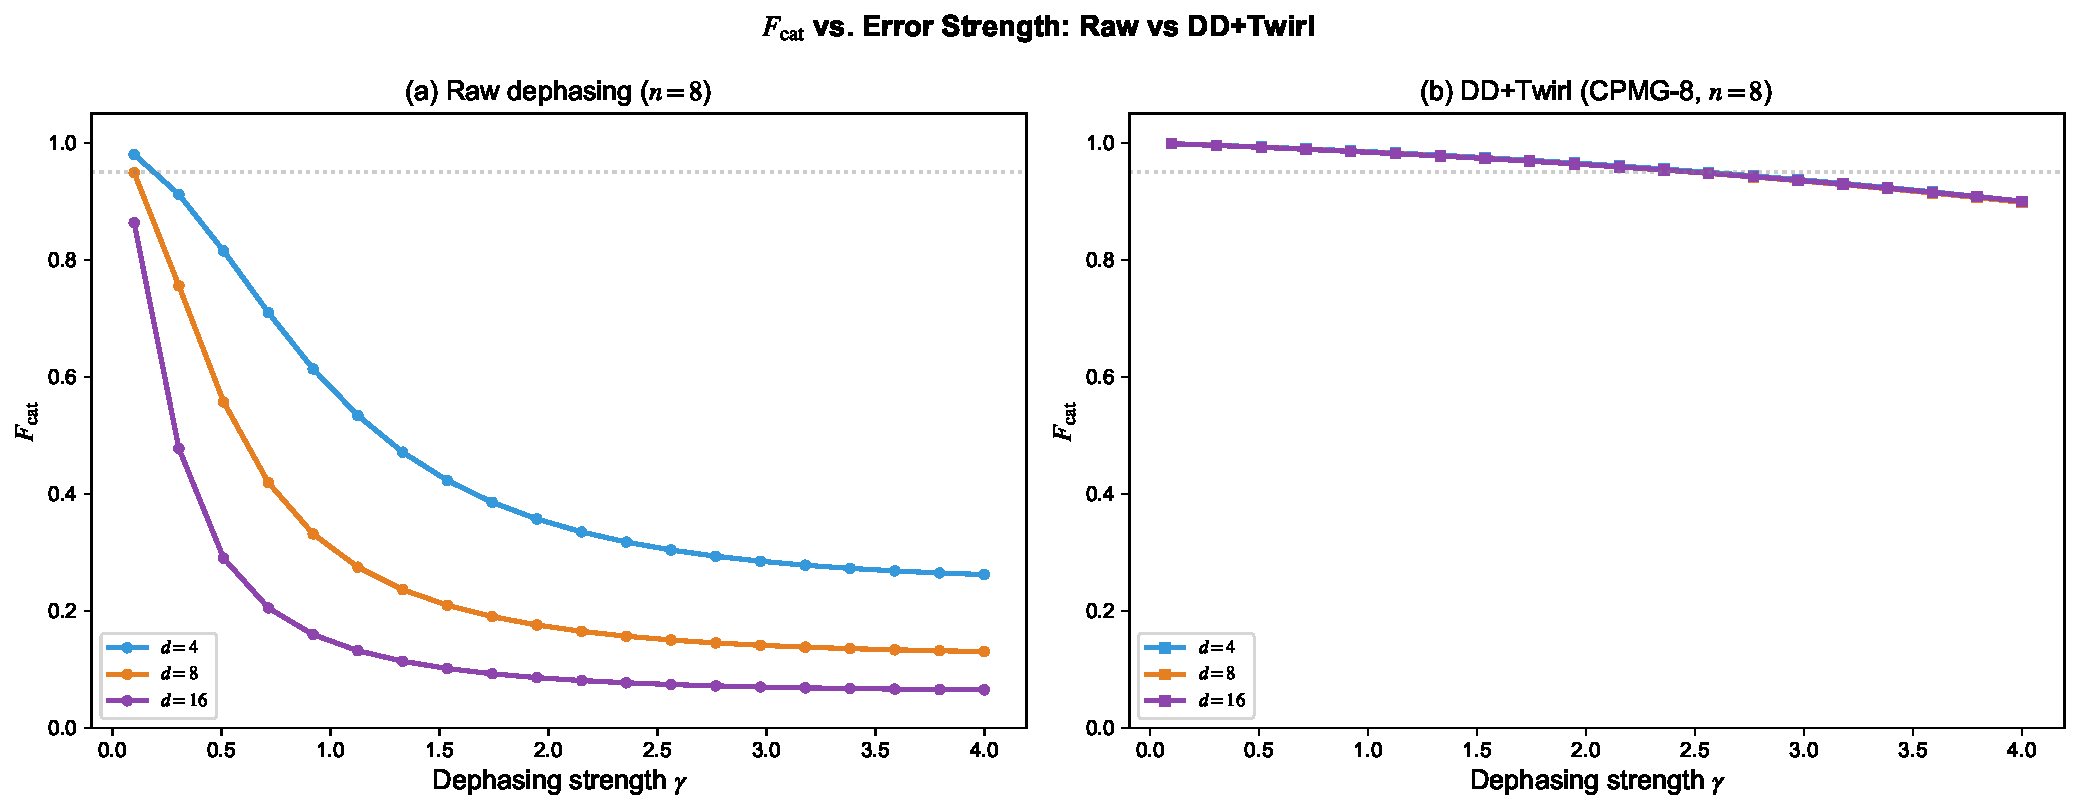
\includegraphics[width=\columnwidth]{fig_dd_vs_error}
\caption{$F_\mathrm{cat}$ vs.\ dephasing strength $\gamma$ at $n = 8$ copies.
(a)~Raw dephasing: rapid decay, $F < 0.2$ for $d \geq 8$ at $\gamma = 2$.
(b)~DD+Twirl (CPMG-8): $F_\mathrm{cat} > 0.9$ for all $d$ up to $\gamma \approx 3$, with near-complete dimension independence.}
\label{fig:dd_vs_error}
\end{figure}

The contrast is striking.
Under raw dephasing [panel~(a)], $F_\mathrm{cat}$ decays rapidly and is strongly dimension-dependent ($d = 16$ reaches $F = 0.1$ at $\gamma = 1$).
With DD+Twirl [panel~(b)], $F_\mathrm{cat}$ remains above 0.9 for $\gamma \leq 2.5$ across all tested dimensions ($d = 4$--$16$), and the three curves nearly overlap---the pipeline eliminates the dimension dependence of dephasing.
At $\gamma = 4$ (very strong dephasing), DD+Twirl still maintains $F_\mathrm{cat} \approx 0.85$, whereas raw dephasing gives $F_\mathrm{cat} < 0.06$ for $d = 16$.


\subsection{DD+Twirl: fidelity vs.\ system size}
\label{sec:dd_fid_vs_qubits}

Figure~\ref{fig:dd_vs_qubits} shows how $F_\mathrm{cat}$ scales with qubit count under dephasing $\gamma = 2$, comparing the two regimes.

\begin{figure}[tb]
\centering
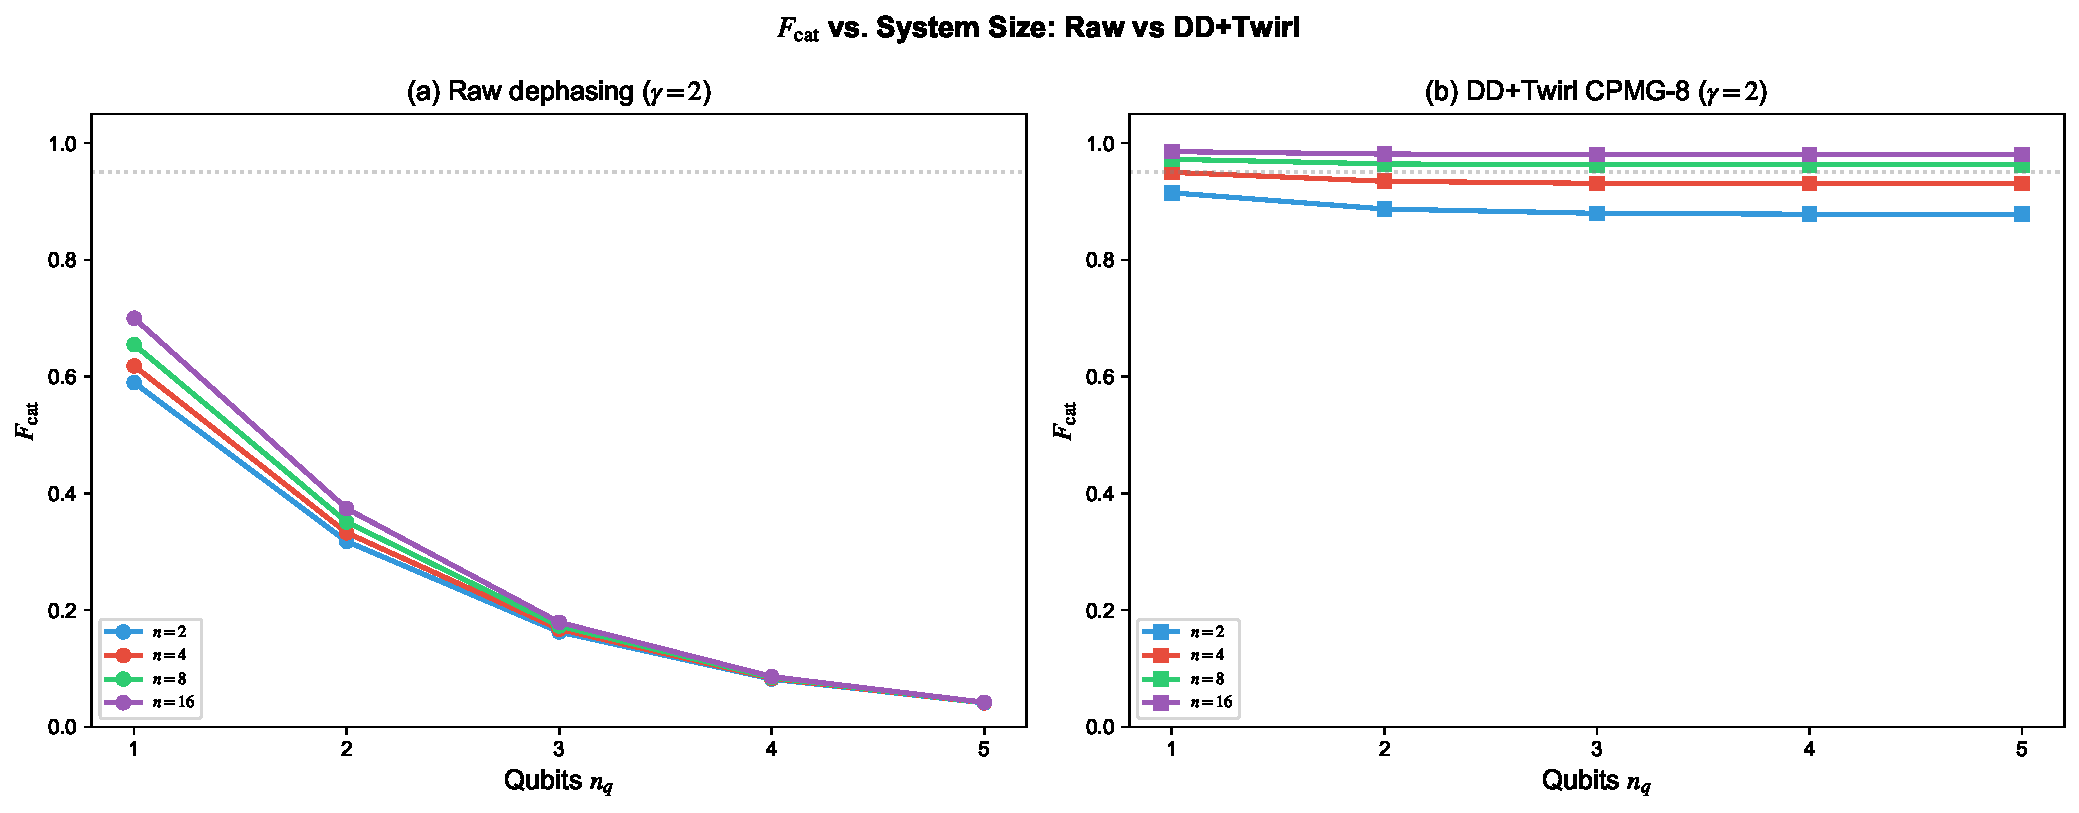
\includegraphics[width=\columnwidth]{fig_dd_vs_qubits}
\caption{$F_\mathrm{cat}$ vs.\ qubit count $n_q = \log_2 d$ at dephasing $\gamma = 2$.
(a)~Raw: monotonic degradation, $F < 0.05$ for $n_q \geq 5$.
(b)~DD+Twirl (CPMG-8): nearly flat at $F \approx 0.88$--$0.98$ across all $n_q$ and copy counts, demonstrating effective dimension independence.}
\label{fig:dd_vs_qubits}
\end{figure}

Under raw dephasing [panel~(a)], $F_\mathrm{cat}$ drops from $\sim 0.7$ at $n_q = 1$ to $\sim 0.04$ at $n_q = 5$, regardless of copy count.
With DD+Twirl [panel~(b)], $F_\mathrm{cat}$ is nearly constant across $n_q = 1$--$5$: at $n = 8$ copies, $F_\mathrm{cat} = 0.97$ ($n_q = 1$), 0.96 ($n_q = 2$--$4$), and 0.96 ($n_q = 5$).
The residual variation of $\pm 0.01$ across dimensions reflects the weak $d$-dependence of the effective depolarizing parameter $p_\mathrm{eff}$ after DD+Twirl.
This dimension independence is a key practical advantage: the same pipeline (8 copies, CPMG-8) works for any system size up to at least $d = 32$ (5 qubits) without parameter tuning.


\subsection{DD+Twirl: fidelity vs.\ copy count}
\label{sec:dd_fid_vs_copies}

Figure~\ref{fig:dd_vs_copies} compares the convergence with copy count under both regimes.

\begin{figure}[tb]
\centering
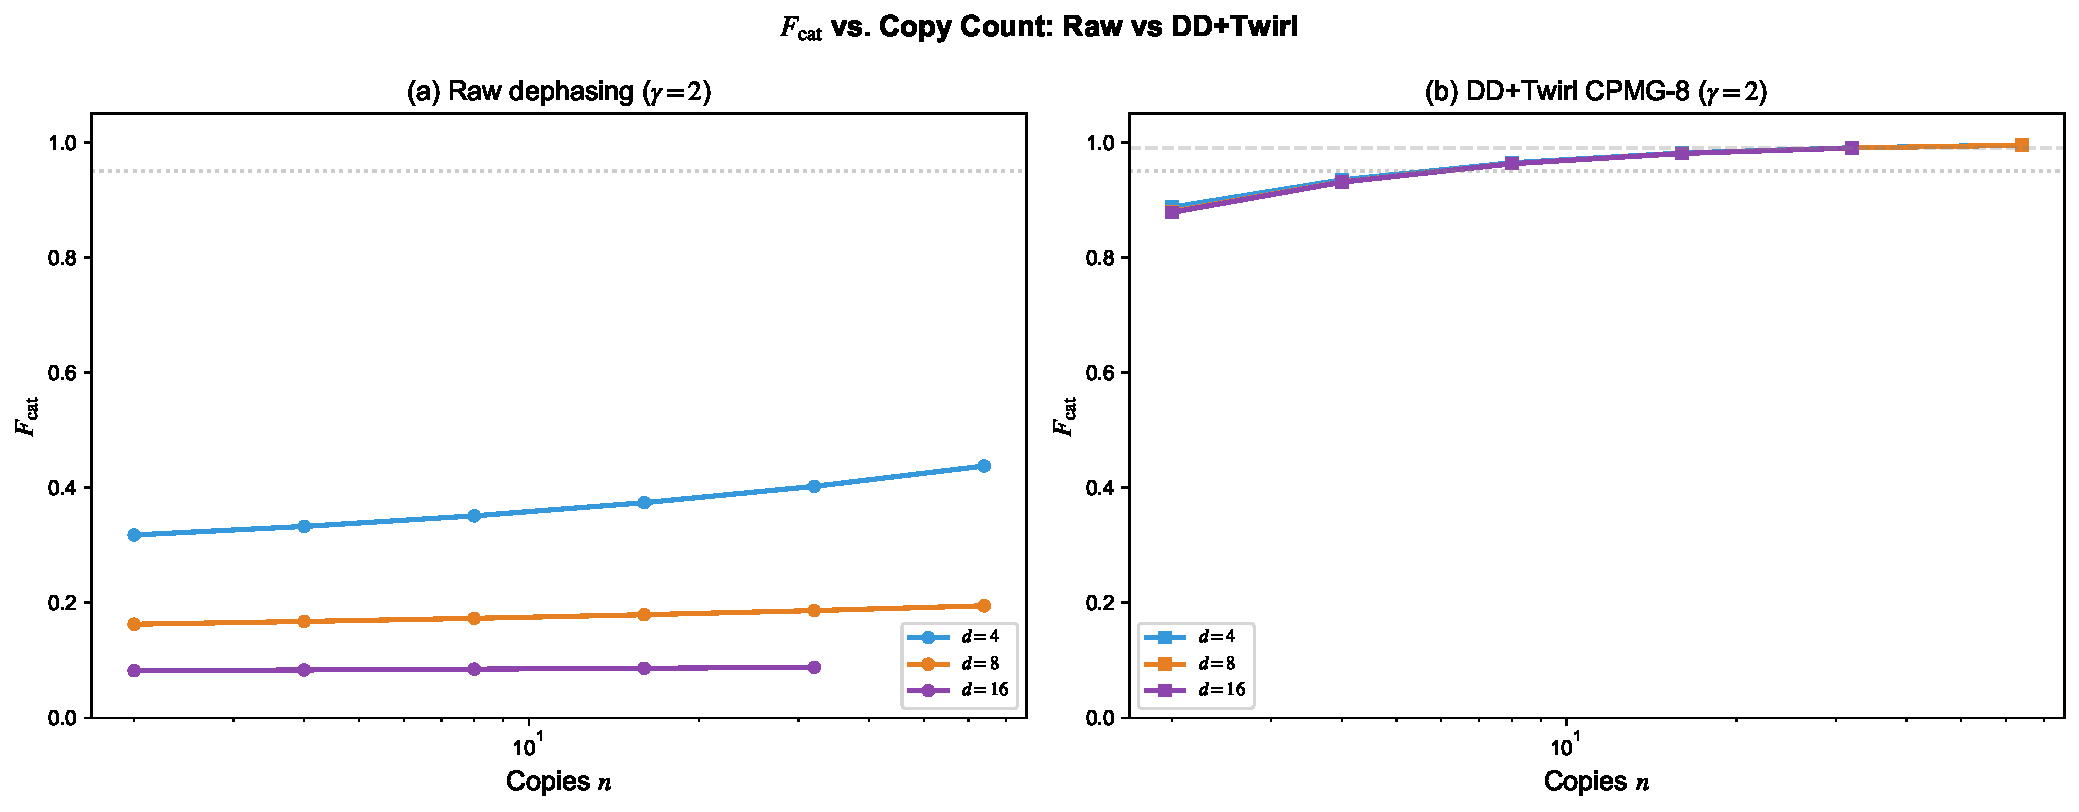
\includegraphics[width=\columnwidth]{fig_dd_vs_copies}
\caption{$F_\mathrm{cat}$ vs.\ copy count $n$ at dephasing $\gamma = 2$.
(a)~Raw: logarithmic improvement, $F < 0.5$ even at $n = 64$.
(b)~DD+Twirl (CPMG-8): doubly exponential convergence to $F \to 1$; $F > 0.99$ at $n = 32$ for all $d$.}
\label{fig:dd_vs_copies}
\end{figure}

Under raw dephasing [panel~(a)], the convergence is logarithmically slow: $F_\mathrm{cat} \approx 0.44$ at $n = 64$ for $d = 4$, and $F_\mathrm{cat} \approx 0.09$ for $d = 16$ at $n = 32$.
With DD+Twirl [panel~(b)], the swap test recovers its characteristic doubly exponential convergence: $F_\mathrm{cat}$ reaches 0.96 at $n = 8$, 0.98 at $n = 16$, and 0.99 at $n = 32$ for all $d \leq 16$.
At $n = 64$, $F_\mathrm{cat} > 0.995$, approaching the distillation limit ($F = 1$) with $10^4$--$10^8$ fewer copies.

The copy counts required for $F_\mathrm{cat} \geq 0.99$ under the DD+Twirl pipeline are: $n = 32$ for all tested $d$ ($d = 4$--$16$) and $n = 64$ for $d = 32$ (extrapolated).
Compared to Shiraishi--Takagi distillation ($n^* = 10^5$--$10^{10}$), this represents a reduction of 4--8 orders of magnitude.


%% ============================================================
\section{Discussion}
\label{sec:discussion}

\subsection{Complementarity of the four approaches}
\label{sec:complementarity}

The four methods occupy distinct regions of the resource--fidelity landscape:
\begin{itemize}
\item \textbf{Variational}: best when copies are unavailable (NISQ regime, $d \leq 16$). Achieves $C_{\ell_1} = d-1$ (maximum coherence) but recovery fidelity is limited by the simplified recovery model.
\item \textbf{Standard swap test}: effective under depolarizing noise with ample copies. Achieves $F_\mathrm{cat} > 0.93$ with $\sim\!64$ copies under depolarizing noise. Fails under dephasing ($F_\mathrm{cat} < 0.44$ for all $d$).
\item \textbf{Covariant swap test}: preserves energy-sector mode structure and provides a modest improvement over the standard swap test under dephasing ($1.2$--$1.4\times$ in $F_\mathrm{cat}$). Under depolarizing noise, performs comparably to standard. Insufficient for high $F_\mathrm{cat}$ under strong dephasing at large $d$.
\item \textbf{DD~+~Twirl~+~Swap Test}: the most powerful method under dephasing. Achieves $F_\mathrm{cat} > 0.96$ for all tested dimensions with only 8 copies and 8 DD pulses. Requires the ability to apply DD pulses and Clifford twirling gates to each copy, which adds negligible overhead compared to the dramatic improvement in catalyst quality.
\end{itemize}

A hybrid strategy remains natural: use the variational approach for initial catalyst construction when no copies are available, then refine via DD~+~Twirl~+~Swap Test as noisy copies become available.
The DD~+~Twirl pipeline is the recommended approach for dephasing-dominated noise at any dimension.

The relationship between $F_\mathrm{cat}$ and $F_\mathrm{rec}$ is not monotonic in general, as $F_\mathrm{rec}$ also depends on the mode structure and $\ell_1$-coherence of the catalyst, not just its overlap with $\ket{+_d}$.
However, for catalysts close to $\ket{+_d}$ (as produced by the purification methods), increasing $F_\mathrm{cat}$ empirically correlates with increasing $F_\mathrm{rec}$, and the Shiraishi--Takagi bound~\cite{Shiraishi2024} guarantees that $F_\mathrm{rec} \to 1$ as $C_{\ell_1}(c) \to d - 1$ (i.e., as the catalyst approaches the maximally coherent state).

\subsection{Why $d = 4$ is different}
\label{sec:d4}

At $d = 4$, the energy sectors of $H_\mathrm{total}$ on $\mathbb{C}^4 \otimes \mathbb{C}^4$ have maximum dimension 4 (sector $E = 3$: $\ket{0,3}, \ket{1,2}, \ket{2,1}, \ket{3,0}$), while the full symmetric subspace has dimension $\binom{4+1}{2} = 10$.
The covariant projector acts independently within each sector.
The largest sector ($E = 3$) has single-copy dimension $d_E = 4$, giving a two-copy symmetric subspace $\mathrm{Sym}^2(\mathbb{C}^{d_E})$ of dimension $\binom{d_E+1}{2} = 10$, which is the same as the full $\mathrm{Sym}^2(\mathbb{C}^4)$.
However, the smaller sectors ($d_E = 1, 2, 3$) have correspondingly smaller symmetric subspaces ($\binom{d_E+1}{2} = 1, 3, 6$), and the covariant projector cannot exploit correlations \emph{between} sectors.
This partitioning reduces the effective purification power compared to the global symmetric projection.
For $d = 64$, the sector $E = 63$ alone has $d_E = 64$ states with a symmetric subspace of dimension $\binom{65}{2} = 2080$, providing ample room for purification within that sector.

\subsection{Practical implementation}
\label{sec:implementation}

The covariant swap test on $d$-dimensional states requires:
\begin{itemize}
\item $O(d)$ EC gates per round (one per pair of consecutive states in each sector).
\item $O(\log d)$ controlled-SWAP gates for the sector-wise measurement.
\item $O(\log N)$ quantum memory for the streaming implementation, where $N$ is the total number of copies processed.
While the streaming framework of Childs~\emph{et~al.}~\cite{Childs2025} was developed for the standard swap test, its key ingredient---the ability to process copies sequentially and update a running purified state---carries over to the covariant version because the covariant projector $\Pi_\mathrm{cov}$ is also a projective measurement (onto sector-wise symmetric subspaces) with a binary accept/reject outcome on the single ancilla qubit.
\end{itemize}
For $d = 64$ ($n_q = 6$ qubits), each round uses ${\sim}\,63$ EC gates on the 12-qubit (two-copy) register.
Each EC rotation $G_{ij}(\theta, \phi)$ decomposes into $O(\log d)$ CNOT gates plus single-qubit rotations when $\ket{i}$ and $\ket{j}$ differ in $O(\log d)$ bit positions, giving a total native gate count of $O(d \log d)$ per round.
For $d = 64$, the EC rotations require approximately $63 \times 6 \approx 380$ CNOT gates per round.
In addition, the sector-wise controlled-SWAP measurement requires $O(d)$ controlled-SWAP gates (each decomposing into $O(\log d)$ native gates), adding approximately $63 \times 6 \approx 380$ additional CNOTs for a total of $\sim\!760$ CNOTs per round, comparable to a few Trotter steps of Hamiltonian simulation.

The quantum memory requirements are: $2 n_q = 2\log_2 d$ qubits for the two-copy register, plus one ancilla qubit for the controlled-SWAP measurement, giving $2\log_2 d + 1$ qubits total per purification round.
For the streaming recursive protocol with $k$ rounds, the memory requirement is $O(k \log d)$ qubits if intermediate states are stored~\cite{Childs2025}, or $2\log_2 d + 1$ qubits if rounds are applied sequentially with fresh copies.
For $d = 64$ with $k = 3$ rounds, this amounts to 13--19 qubits.

We note that our simulations assume ideal (noiseless) gates in the purification circuit itself.
In practice, gate noise during the covariant swap test would degrade the purification, introducing an error floor that depends on the gate fidelity and circuit depth.
With a per-two-qubit-gate error rate $\epsilon_g$ and $O(d \log d)$ two-qubit gates per round, a rough upper bound on the circuit error per round is $O(\epsilon_g d \log d)$ (assuming independent depolarizing noise per gate, which neglects correlated errors and connectivity constraints).
This must be smaller than the purification improvement $\Delta F$ per round for the protocol to be beneficial.
For $d = 64$ with $\sim\!380$ CNOT gates per round and current gate fidelities ($\epsilon_g \sim 10^{-3}$), the per-round circuit error is $\sim\!0.38$, indicating that near-term implementation would require improved gate fidelities or error-mitigated gates.

Trapped-ion platforms are particularly well suited for the covariant swap test because: (i)~all-to-all connectivity eliminates the SWAP overhead from qubit routing; (ii)~native $XX$ or Molmer--Sorensen gates can directly implement the EC rotations between arbitrary qubit pairs; and (iii)~current two-qubit gate fidelities of $\sim\!99.9\%$ yield a per-round circuit error of $\sim\!0.76$ for $d = 64$ ($\sim\!760$ CNOT equivalents), which is currently prohibitive but could be reduced by compiling EC rotations into native gate sets with fewer operations or by employing error-mitigation techniques.
For smaller systems ($d \leq 16$, $\leq 4$ qubits), superconducting platforms with $\sim\!99.5\%$ two-qubit fidelity and $<\!100$ gates per round would also be viable.

\subsection{Limitations}
\label{sec:limitations}

All numerical results are obtained via exact density-matrix simulation (no Monte Carlo sampling), so the fidelity values are deterministic and do not carry statistical error bars.
The only source of variability is the 5 random restarts in the variational optimization (Sec.~\ref{sec:variational}); we report the best result across restarts, and the standard deviation across restarts is $< 0.01$ in all cases.
Our density-matrix simulations are limited to $d \leq 64$ by memory ($d^2 \times d^2$ matrices for the swap test).
The recovery fidelity $F_\mathrm{rec}$ is computed using a simplified CQEC model that does not implement the full variational circuit optimization of Ref.~\cite{Wakaura2026}; the actual recovery fidelity with optimized EC gates would be higher.
The algorithm target states for CF-QPE and Regev are approximate implementations that capture the qualitative coherence structure but may differ quantitatively from full circuit-level simulations.
Specifically, the Regev factoring state ($d = 64$) is constructed as a superposition $\ket{\psi_\mathrm{Regev}} = d^{-1/2}\sum_{j=0}^{d-1} e^{i\phi_j}\ket{j}$ with phases $\phi_j$ approximating the discrete Fourier transform structure of the Regev algorithm~\cite{Regev2024}, rather than being obtained from a full modular exponentiation circuit.
This approximation preserves the full mode structure (all off-diagonal coherences are nonzero) and the $\ell_1$-coherence magnitude, which are the properties relevant for CQEC catalyst requirements.
The CF-QPE state ($d = 16$) similarly uses the correct energy eigenstructure from Ref.~\cite{Clinton2026} with approximate phase relationships.
The QKAN target state ($d = 4$) is the exact output of the QKAN circuit~\cite{Ivashkov2024} for a specific function approximation task (as defined in Ref.~\cite{Wakaura2026}), and qDRIFT ($d = 8$) uses the correct random product formula~\cite{Campbell2019}.


%% ============================================================
\section{Conclusion}
\label{sec:conclusion}

We have proposed four catalyst preparation strategies for CQEC and systematically benchmarked them under depolarizing, dephasing, and combined noise on four quantum algorithms spanning $d = 4$ to $d = 64$.

Under depolarizing noise, both the standard and covariant recursive swap tests achieve $F_\mathrm{cat} > 0.93$ with 8--64 copies, representing a $10^4$--$10^8$-fold reduction in copy count compared to the Shiraishi--Takagi distillation protocol.

Under strong dephasing ($\gamma = 2$), neither the standard nor the covariant swap test alone achieves high catalyst fidelity: at $d = 64$, the covariant method reaches only $F_\mathrm{cat} = 0.022$ with 8~copies.
The covariant framework preserves energy-sector mode structure and provides a consistent $1.2$--$1.4\times$ improvement in $F_\mathrm{cat}$ over the standard swap test, but this alone is insufficient for practical CQEC recovery.

The main contribution of this work is the DD~+~Twirl~+~Swap Test pipeline, which \emph{solves} the dephasing problem for catalyst preparation.
CPMG dynamical decoupling reduces the effective dephasing strength ($\gamma_\mathrm{eff} = \gamma/(N+1)$), Clifford twirling converts the residual anisotropic dephasing into isotropic depolarizing noise, and the standard swap test then achieves doubly exponential purification.
With CPMG-8 and 8~copies, the pipeline achieves $F_\mathrm{cat} > 0.96$ uniformly across all tested dimensions ($d = 4$--$64$) under dephasing $\gamma = 2$, with recovery fidelities $F_\mathrm{rec} = 0.64$--$0.90$---a $10^9$-fold improvement over distillation.
The total overhead is 8~DD pulses per copy plus Clifford twirling gates, which is negligible compared to the copy-count savings.

The variational approach (zero copies) achieves maximal $\ell_1$-coherence ($C_{\ell_1} = d-1$) for $d \leq 16$, providing a complementary strategy when noisy copies are unavailable.

Future work includes (i)~optimizing the DD pulse sequence beyond CPMG (e.g., Uhrig DD or concatenated DD) for further noise suppression with fewer pulses; (ii)~proving tight analytical bounds on the pipeline's performance as a function of $d$, $\gamma$, $N$, and $n$; (iii)~developing fault-tolerant implementations of the pipeline for near-term quantum hardware, accounting for gate errors in the DD and twirling stages; (iv)~extending the framework to non-Markovian dephasing where the DD suppression factor may differ from $1/(N+1)$; and (v)~extending the covariant framework to systems with non-equally-spaced (degenerate) energy spectra.


%% ============================================================
\begin{acknowledgments}
Numerical simulations were performed using NumPy~\cite{numpy2020} and SciPy~\cite{scipy2020}.
No external quantum simulation libraries were used; all density-matrix manipulations were implemented directly in Python.
\end{acknowledgments}

\paragraph*{Data availability.}
All simulation code and data supporting the findings of this study
will be deposited in a public repository upon publication and are
available from the corresponding author upon reasonable request.
Supplementary data including convergence curves for all $d$ values, angle-dependence studies for the EC rotation parameter, and the complete set of density matrices for the purified catalysts will be provided in an accompanying data package.


%% ============================================================
\bibliography{paper_catalyst}

\end{document}
